% !Mode:: "TeX:DE:UTF-8:Main"

\documentclass{beamer}\usepackage[]{graphicx}\usepackage[]{color}
%% maxwidth is the original width if it is less than linewidth
%% otherwise use linewidth (to make sure the graphics do not exceed the margin)
\makeatletter
\def\maxwidth{ %
  \ifdim\Gin@nat@width>\linewidth
    \linewidth
  \else
    \Gin@nat@width
  \fi
}
\makeatother

\definecolor{fgcolor}{rgb}{0.345, 0.345, 0.345}
\newcommand{\hlnum}[1]{\textcolor[rgb]{0.686,0.059,0.569}{#1}}%
\newcommand{\hlstr}[1]{\textcolor[rgb]{0.192,0.494,0.8}{#1}}%
\newcommand{\hlcom}[1]{\textcolor[rgb]{0.678,0.584,0.686}{\textit{#1}}}%
\newcommand{\hlopt}[1]{\textcolor[rgb]{0,0,0}{#1}}%
\newcommand{\hlstd}[1]{\textcolor[rgb]{0.345,0.345,0.345}{#1}}%
\newcommand{\hlkwa}[1]{\textcolor[rgb]{0.161,0.373,0.58}{\textbf{#1}}}%
\newcommand{\hlkwb}[1]{\textcolor[rgb]{0.69,0.353,0.396}{#1}}%
\newcommand{\hlkwc}[1]{\textcolor[rgb]{0.333,0.667,0.333}{#1}}%
\newcommand{\hlkwd}[1]{\textcolor[rgb]{0.737,0.353,0.396}{\textbf{#1}}}%
\let\hlipl\hlkwb

\usepackage{framed}
\makeatletter
\newenvironment{kframe}{%
 \def\at@end@of@kframe{}%
 \ifinner\ifhmode%
  \def\at@end@of@kframe{\end{minipage}}%
  \begin{minipage}{\columnwidth}%
 \fi\fi%
 \def\FrameCommand##1{\hskip\@totalleftmargin \hskip-\fboxsep
 \colorbox{shadecolor}{##1}\hskip-\fboxsep
     % There is no \\@totalrightmargin, so:
     \hskip-\linewidth \hskip-\@totalleftmargin \hskip\columnwidth}%
 \MakeFramed {\advance\hsize-\width
   \@totalleftmargin\z@ \linewidth\hsize
   \@setminipage}}%
 {\par\unskip\endMakeFramed%
 \at@end@of@kframe}
\makeatother

\definecolor{shadecolor}{rgb}{.97, .97, .97}
\definecolor{messagecolor}{rgb}{0, 0, 0}
\definecolor{warningcolor}{rgb}{1, 0, 1}
\definecolor{errorcolor}{rgb}{1, 0, 0}
\newenvironment{knitrout}{}{} % an empty environment to be redefined in TeX

\usepackage{alltt}
\usepackage{tikz}
\usepackage[english]{babel}
\usepackage[utf8]{inputenc}
\usepackage[T1]{fontenc}
\usepackage{lipsum}

\usepackage{textpos} 
\usepackage{hyperref}
\usepackage{amsmath,amsthm,amsfonts,nicefrac,mathabx,amssymb}
\usepackage[subnum]{cases}
\usepackage{calligra, mathrsfs}
%\usepackage{natbib}
\usepackage{booktabs}
%\bibpunct{(}{)}{;}{a}{,}{,}

\usepackage{helvet}
\usepackage{graphicx}
\usepackage{color}
\usepackage{multirow,dcolumn}
\usepackage{ragged2e}
\usepackage{xcolor}
\usepackage{colortbl}
\usepackage{booktabs}
\usepackage{url}
\usepackage{bibentry}
\usepackage{chngcntr}

\usepackage{animate} %for animation

\usetheme{Gesis}


\newcommand{\eqname}[1]{\tag*{#1}} %equation title

%new math cal fonds
\newenvironment{frcseries}{\fontfamily{frc}\selectfont}{}
\newcommand{\textfrc}[1]{{\frcseries#1}}
\newcommand{\mathfrc}[1]{\text{\textfrc{#1}}}

\setcounter{tocdepth}{1}
\setbeamercolor*{section in toc}{fg=hellgrau}
\setbeamertemplate{bibliography item}[default]


\setcounter{secnumdepth}{3}
\setcounter{tocdepth}{3}


\newcommand{\E}[1]{\text{E}\left(#1\right)}
\newcommand{\V}[1]{\text{V}\left(#1\right)}
\newcommand{\Vest}[1]{\widehat{\text{V}}\left(#1\right)}
\newcommand{\MSE}[1]{\text{MSE}\left(#1\right)}
\newcommand{\COV}[2]{\text{COV}\left(#1,\,#2\right)}

\newcommand{\RN}[1]{%
  \textup{\uppercase\expandafter{\romannumeral#1}}%
}


\makeatletter

%%%%%%%%%%%%%%%%%%%%%%%%%%%%%% LyX specific LaTeX commands.
\providecommand{\LyX}{\texorpdfstring%
  {L\kern-.1667em\lower.25em\hbox{Y}\kern-.125emX\@}
  {LyX}}

%%%%%%%%%%%%%%%%%%%%%%%%%%%%% Textclass specific LaTeX commands.
% this default might be overridden by plain title style
 \newcommand\makebeamertitle{\frame{\maketitle}}%
 % (ERT) argument for the TOC
 \AtBeginDocument{%
   \let\origtableofcontents=\tableofcontents
   \def\tableofcontents{\@ifnextchar[{\origtableofcontents}{\gobbletableofcontents}}
   \def\gobbletableofcontents#1{\origtableofcontents}
 }

% A Section Title Slides
\AtBeginSection{\frame{\sectionpage}}
\AtBeginSubsection{\frame{\subsectionpage}}


\title{Sample Theory}
\subtitle{Epidemiological Study Design and Statistical Methods}

\author{Stefan Zins - GESIS}
\date{12.12.2017}

% Gestaltungsvarianten
% Kopfbandfarbe "shaded" von weiß zu blau: 
% \setbeamertemplate{gesisheadband}[shaded]
% andere Farbwerte
% \gesisCIbluecolors % = Blau und Orange aus CI, Blau als heller Hintergrund
% \gesisCIcolors     % = Blau und Orange aus CI, Sand als heller Hintergrund



%
% knitr setup 
% ------------------------------------------------------------------------------   


\IfFileExists{upquote.sty}{\usepackage{upquote}}{}
\begin{document}

\gesismaketitle % erzeugt Titelseite

\begin{frame}%[t]
  \frametitle{Content}
  
  \begin{itemize}
  \item Design Based Inference
  \item Sampling Designs
  \item Sample Size Planning
  \end{itemize}


\emph{SamplignAndEstimation} on GitHub, branch sampling\_short:
\url{https://github.com/BernStZi/SamplingAndEstimation/tree/sampling_short}
\end{frame}


\begin{frame}{Motivation}
 \begin{itemize}
    \item<1>  Did you ever work with sample data? 
    \item<2> What kind of analysis have you done with sample data?
    \item<3>  What concerns did you have while applying your analytically methods?
  \end{itemize}
\end{frame}



\section{Design Based Inference}



\begin{frame}{\alert{Finite} Population, Sample, and Sampling Design}

 \begin{itemize}
 \item[] 
 \begin{align}
 \mathcal{Y} = & \{ y_1{,}y_2{,}\,\ldots{,}\,y_k{,}\,\ldots{,}\,y_N \} \eqname{finite population of size $N$} \\
 \mathcal{U} = &\, \{ 1{,}2{,}\,\ldots{,}\,k{,}\,\ldots{,}\,N \} \eqname{sampling frame} \\
 \mathfrc{s} \subset &\, \mathcal{U} \eqname{sample of size $n$} \\
 \mathcal{P}(\mathcal{U}) & \eqname{all possible subsets of $\mathcal{U}$}
 \end{align}
 \item[] The discrete probability distribution $p(.)$ over $\mathcal{P}(\mathcal{U})$ is called a \emph{sampling design} and  $\mathcal{G}=\{ \mathfrc{s} | \mathfrc{s} \in \mathcal{P}(\mathcal{U}),\, p(\mathfrc{s}) > 0 \}$ is called the support of $p(.)$ with
$$
\sum_{\mathfrc{s} \in \mathcal{G}} p(\mathfrc{s}) = 1\;.
$$
 \end{itemize}
\end{frame}


\begin{frame}{Estimation}
\begin{align}
 \theta       & = f(\mathcal{Y})  \eqname{statistic of interest} \\
 \hat{\theta} & = f(\mathcal{Y}, \mathfrc{s} )  \eqname{estimator for $\theta$} \\
 \E{\hat{\theta}} & = \sum_{\mathfrc{s} \in \mathcal{G}} p(\mathfrc{s}) f(\mathcal{Y}, \mathfrc{s} )   \eqname{expected value of $\hat{\theta}$} \\
 \V{\hat{\theta}}   & =  \E{\hat{\theta}^2} -  {\E{\hat{\theta}}}^2 \eqname{variance of  $\hat{\theta}$} 
\end{align}
 $\E{.}$ and $\V{.}$ are always with respect to the sampling design $p()$ and
 an estimator is said to be unbiased if
 $$ \E{\hat{\theta}} = \theta\;. $$
\end{frame}

\begin{frame}{Law of Large Numbers (LLN)}
Weak law of large numbers: 

Suppose $ \{ y_1{,}y_2{,}\,\ldots{,}\,y_k{,}\,\ldots{,}\,y_N \}$ is a sequence of i.i.d. random variables with mean $\mu$ and $\mu \neq \infty$ and $\mu \neq -\infty$. Then for $n \rightarrow \infty$ then we have:

$$
\bar{y} \xrightarrow{P} \mu
$$

If the LLN holds we can have unbiased estimates, as our estimates will converge in probability to their expected (true) value. That is, it assures $\E{I_k}=\pi_k$.
\end{frame}


\begin{frame}{LLN Demonstration}
\onslide*<1>{
Suppose all $y_i$ follow an exponential distribution with mean and variance equal to one. We take repeatedly a sample of size $50$. For each sample the sample mean is calculated. The mean of the sample means should converge towards the true mean of the distribution with increasing number of samples.
}
\onslide<2>{
\begin{knitrout}
\definecolor{shadecolor}{rgb}{0.969, 0.969, 0.969}\color{fgcolor}

{\centering 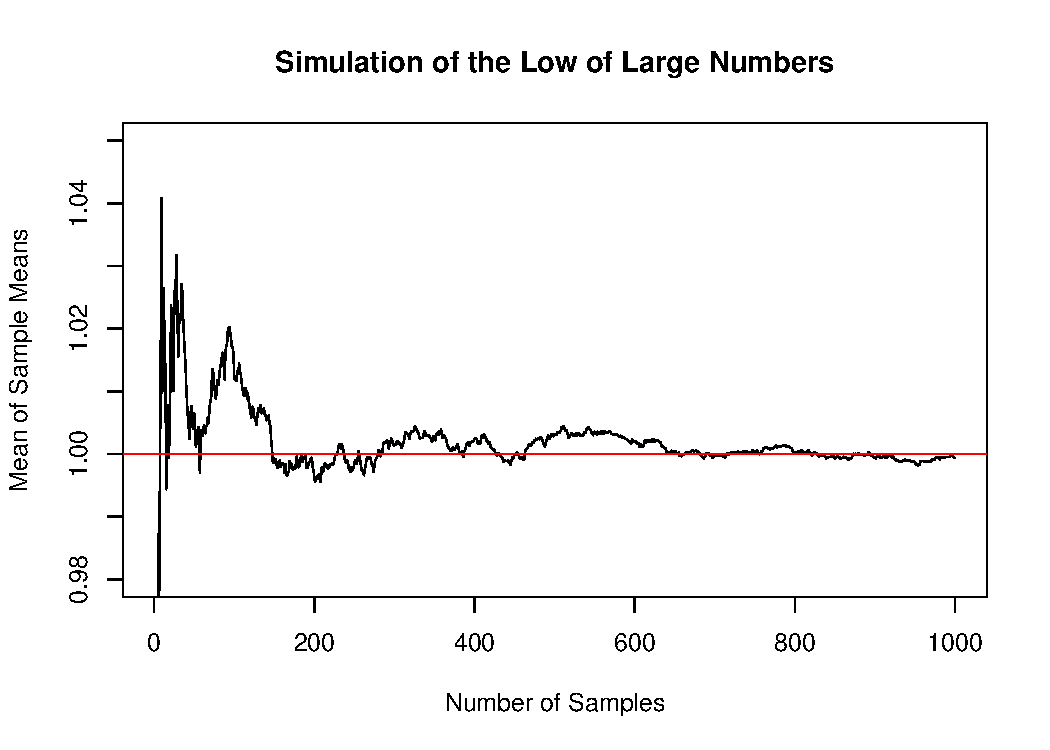
\includegraphics[width=.8\linewidth]{figure/LLN-1} 

}



\end{knitrout}
}
\end{frame}

\begin{frame}{Central  Limit Theorem (CLT)}
CLT of \emph{Lindeberg–L\'evy}: \\
Suppose $\{ y_1{,}y_2{,}\,\ldots{,}\,y_k{,}\,\ldots{,}\,y_N \}$ is a sequence of i.i.d. random variables with $V(y_i) < \infty\;\forall\; i=1,\,\ldots,\,N$. Then for $n \rightarrow \infty$ then we have:
$$
\dfrac{\bar{y}-\mu}{\sigma \sqrt {n}} \ {\xrightarrow {d}}\ N\left(0,1\right)
$$
If the CLT holds, symmetric confidence intervals can be constructed with quantiles from the standard normal distribution $\Phi(z)$
$$
\left[ \bar{y} + \Phi(\alpha/2)\sigma\sqrt{n} \,;\, \bar{y} + \Phi(1-\alpha/2)\sigma\sqrt{n}\right]
$$

%driven by sample size
\end{frame}


\begin{frame}{CLT Demonstration}



\onslide*<1>{
Suppose all $y_i$ follow an exponential distribution with mean and variance equal to one.
\begin{knitrout}
\definecolor{shadecolor}{rgb}{0.969, 0.969, 0.969}\color{fgcolor}

{\centering 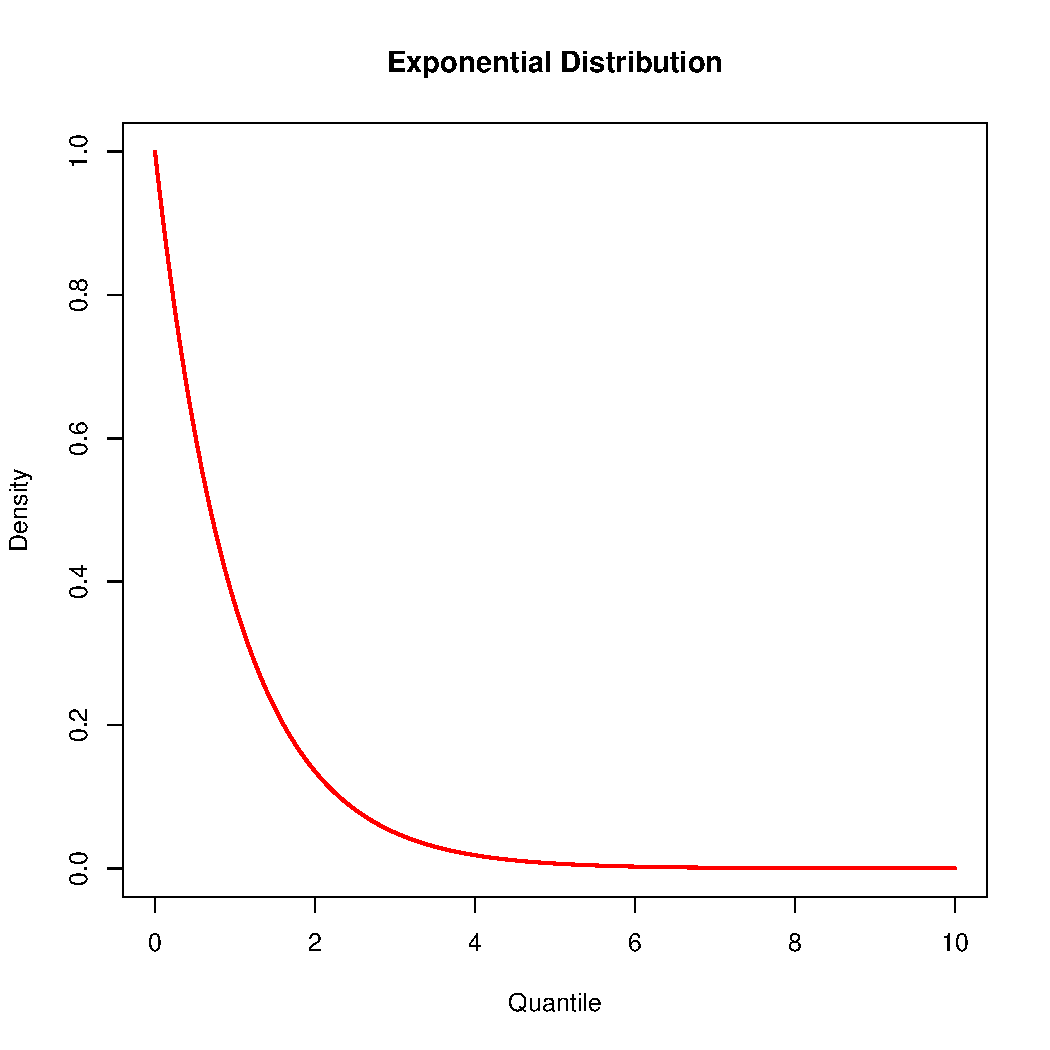
\includegraphics[width=\maxwidth,height=5cm]{figure/CLT_1-1} 

}



\end{knitrout}
}

\onslide*<2>{
\begin{knitrout}
\definecolor{shadecolor}{rgb}{0.969, 0.969, 0.969}\color{fgcolor}

{\centering 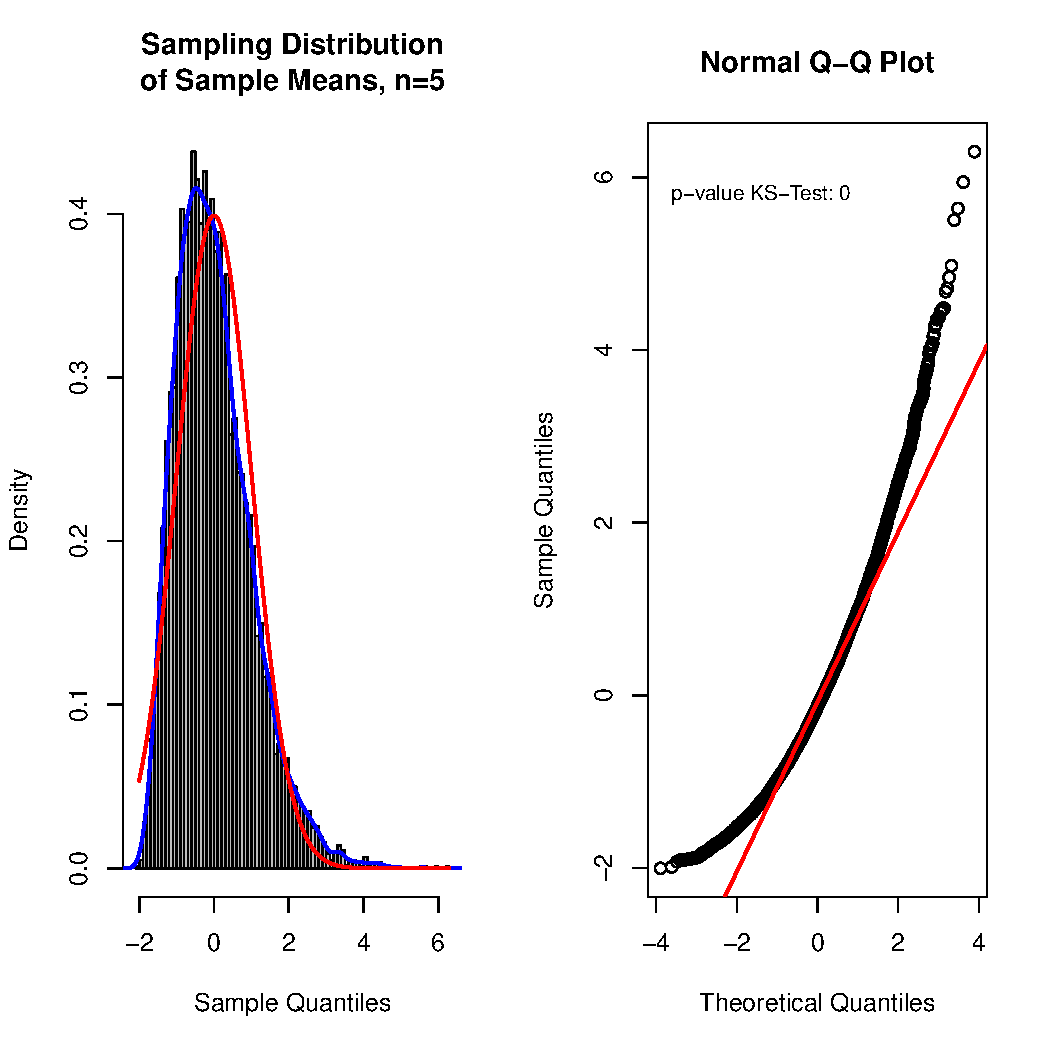
\includegraphics[width=\maxwidth,height=6.75cm]{figure/CLT_2-1} 

}



\end{knitrout}
 }

 \onslide*<3>{
\begin{knitrout}
\definecolor{shadecolor}{rgb}{0.969, 0.969, 0.969}\color{fgcolor}

{\centering 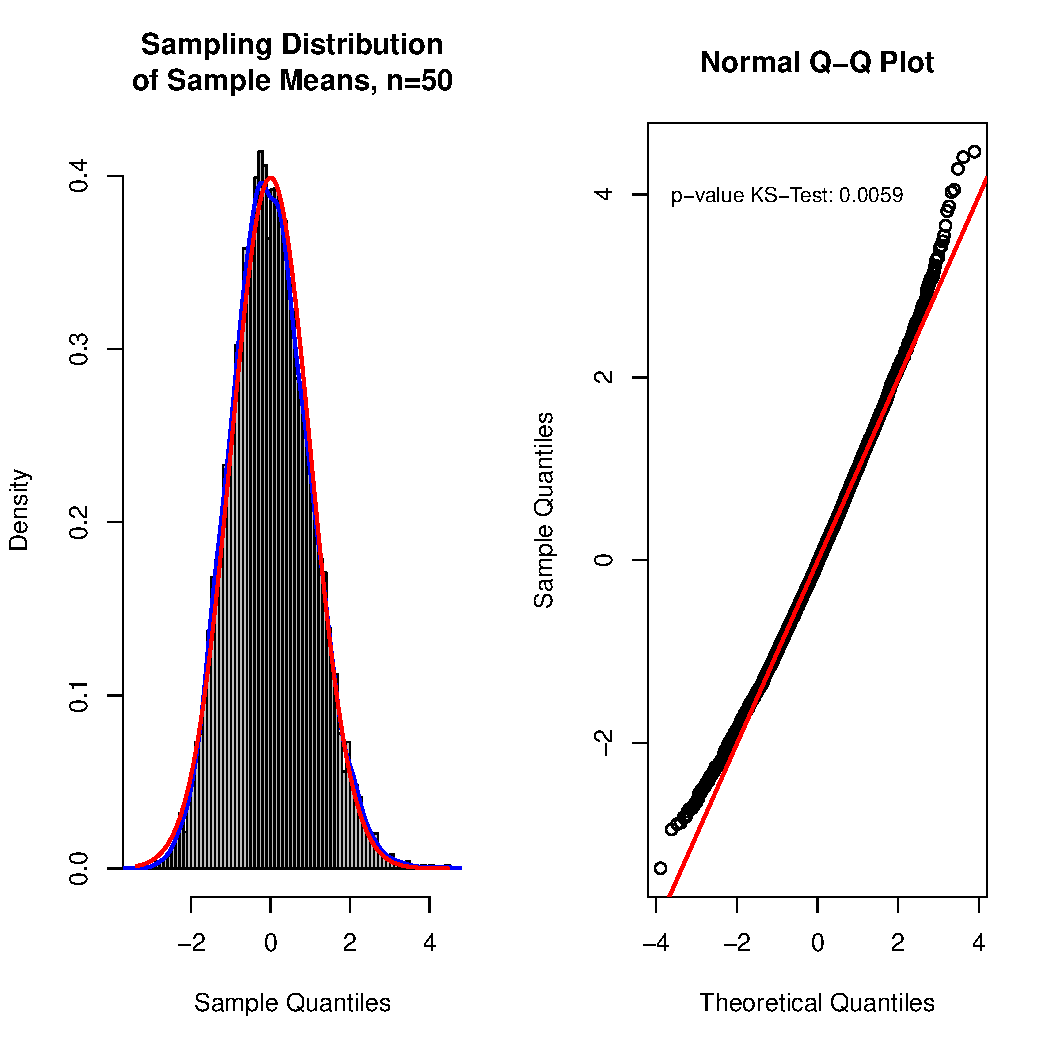
\includegraphics[width=\maxwidth,height=6.75cm]{figure/CLT_3-1} 

}



\end{knitrout}
 }

\onslide*<4>{
\begin{knitrout}
\definecolor{shadecolor}{rgb}{0.969, 0.969, 0.969}\color{fgcolor}

{\centering 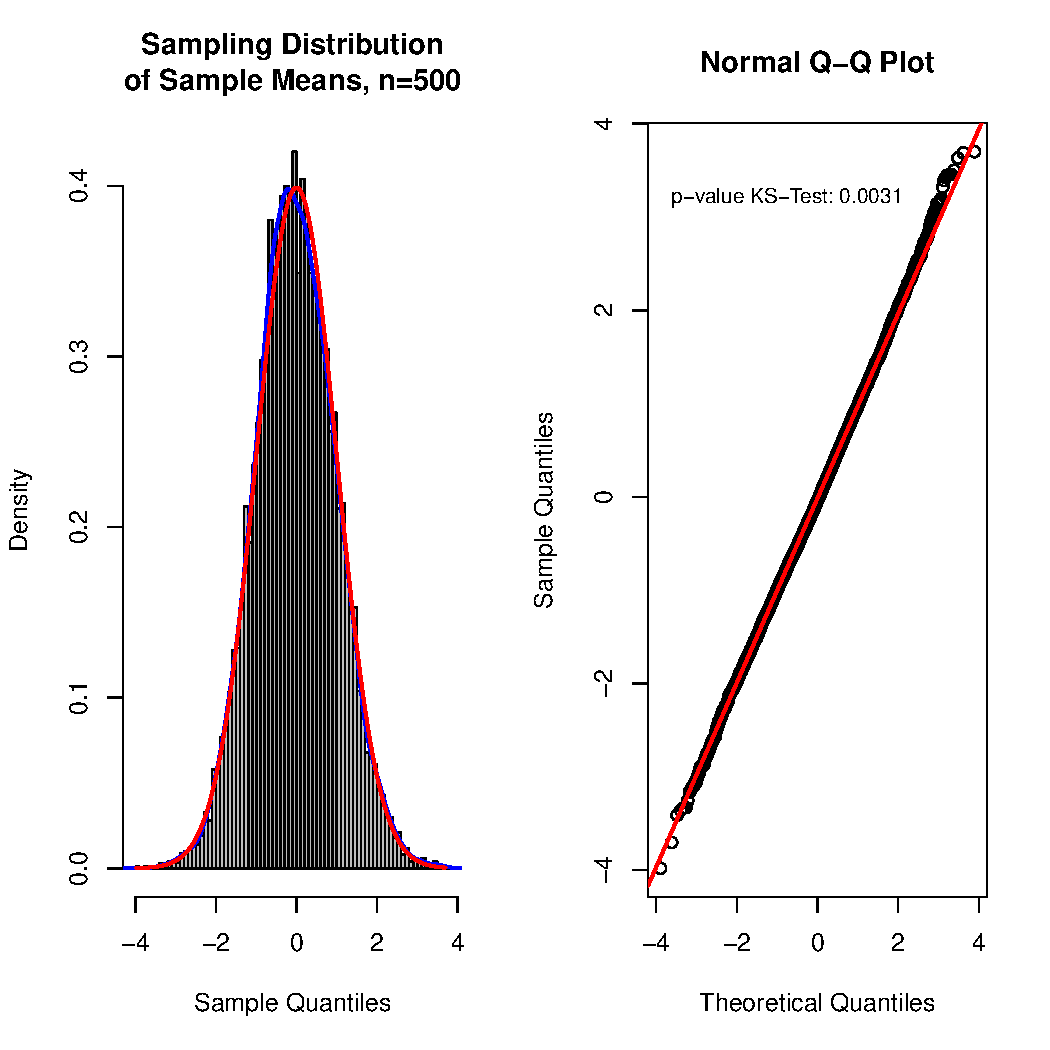
\includegraphics[width=\maxwidth,height=6.75cm]{figure/CLT_4-1} 

}



\end{knitrout}
}
\onslide*<5>{
\begin{knitrout}
\definecolor{shadecolor}{rgb}{0.969, 0.969, 0.969}\color{fgcolor}

{\centering 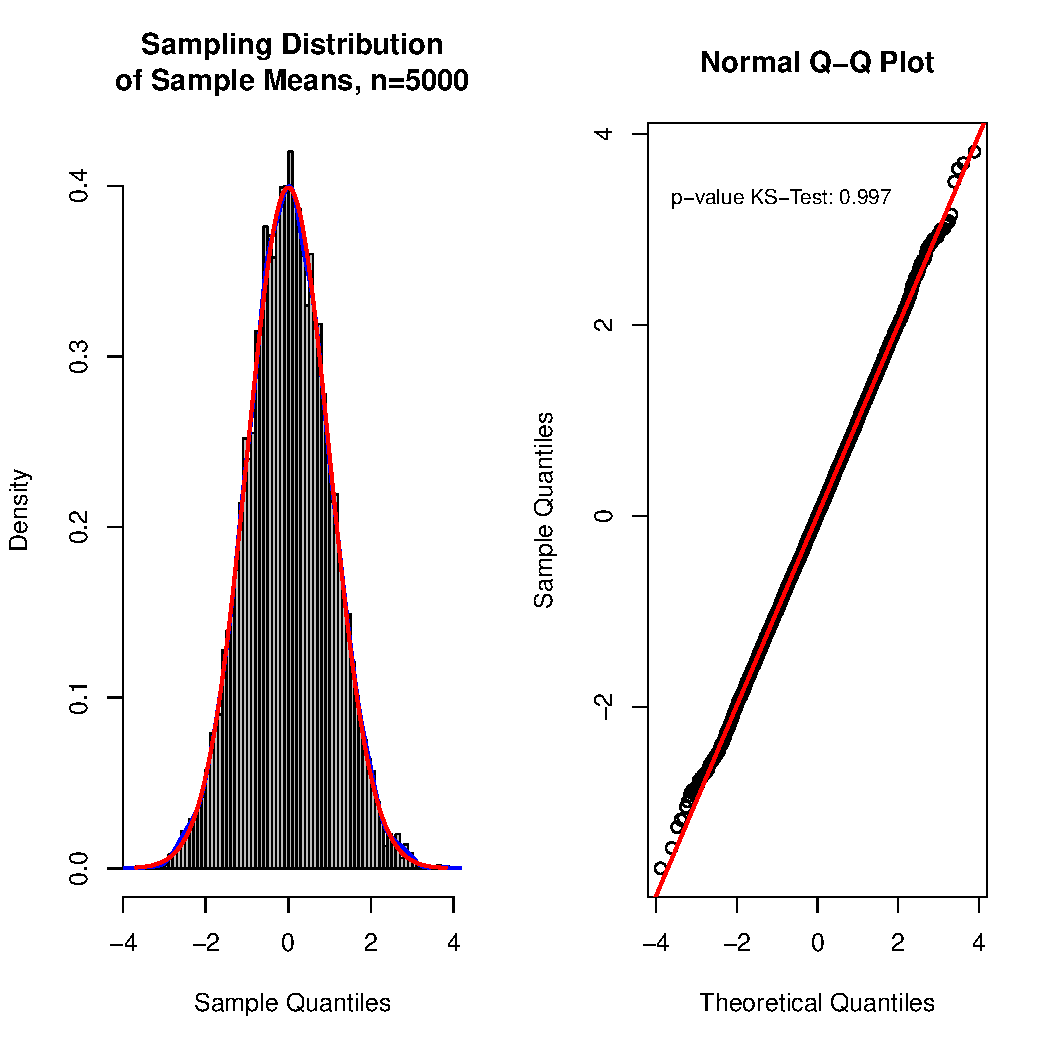
\includegraphics[width=\maxwidth,height=6.75cm]{figure/CLT_5-1} 

}



\end{knitrout}
}
\end{frame}

\begin{frame}{Inclusion Probabilities}
\begin{align}
 I_k   &=   \begin{cases}   1  & \text{if}\; k \in \mathfrc{s} \\
                            0  & \text{else}  
          \end{cases}   \eqname{sampling indicator element $k$} \\
\E{I_k}     &  =   \pi_k    \eqname{inclusion probability of element $k$ } \\
\E{I_k I_l} &  =   \pi_{kl}  \eqname{joint expectation of $I_k$ and $I_l$} \\
\sum_{k \in \mathcal{U}}\pi_k & = \E{n} \eqname{expected sample size}
\end{align}

The $I_k$ are the \emph{only} random variables in the design based frame work and they follow a theoretical distribution. E.g. a Hypergeometric distribution for SRS. 

\end{frame}

\begin{frame}{Inclusion Probabilities}
With the inclusion probabilities design unbiased estimators can be constructed. For example an estimator for a total $\tau=\sum_{k \in \mathcal{U}} y_k$.
\begin{align*}
 \hat\tau &= \sum_{k \in \mathfrc{s}} \dfrac{y_k}{\pi_k} & \E{\hat\tau } &= \sum_{k \in \mathcal{U}} E(I_k) \dfrac{y_k}{\pi_k} = \tau
\end{align*}
$\pi_k^{-1}$ is also called the \alert{design weight} of element $k$.
% Many estimator can be written as functions of totals, which makes it possible to have at least design consistent estimtors for them.

$V(\hat\theta)=f(\mathcal{Y},\Sigma)$, with $\Sigma=(\E{I_k I_l}-\E{I_k} \E{I_l})_{k,l=1,\ldots,N}$.
For complex sampling designs $\Sigma$ can be very complex too and difficult to compute. In practice it is thus often unknown to data users. However there are approximations to $V(\hat\theta)$ that only require the $\pi_k$'s and are much simpler to estimate than $V(\hat\theta)$.

\end{frame}


\begin{frame}{Sample Mean with SRS}
  \small
  \begin{align*} 
  \mu = \dfrac{1}{N} \sum_{k \in \mathcal{U}}  y_k{,}  && \overline{y} = \sum_{k \in \mathfrc{s}}  \dfrac{y_k}{n}{,} && \sigma^2 = \dfrac{1}{N}\sum_{k \in \mathcal{U}} (y_k - \mu )^2{,}
  && V^2 = \sigma^2 \dfrac{N}{N-1}
  \end{align*}
  ~\\[-0.5cm]
  \begin{columns}[t]
   \onslide<2->{
    \begin{column}{.5\textwidth}
      \begin{align*} 
        \E{\overline{y}} & = \E{\sum_{k \in \mathcal{U}} I_k \dfrac{y_k}{n} } \\
        & = \dfrac{1}{n} \sum_{k \in \mathcal{U}} \E{I_k} y_k  \\
        & = \dfrac{1}{n} \sum_{k \in \mathcal{U}} \pi_k y_k  \\
        & = \dfrac{1}{N} \sum_{k \in \mathcal{U}}  y_k  
       \end{align*}
      \end{column}
    \begin{column}{.5\textwidth}
   }
   \onslide<3>{
      \begin{align*} 
        \V{\overline{y}} & = \V{\sum_{k \in \mathcal{U}} I_k \dfrac{y_k}{n}} \\
        & = \dfrac{1}{n^2} \sum_{k \in \mathcal{U}} \sum_{l \in \mathcal{U}} \COV{I_k}{I_l} y_k y_l  \\
        & = -\dfrac{1}{2} \dfrac{1}{n^2} \sum_{k \in \mathcal{U}} \sum_{l \in \mathcal{U}} (\pi_{kl}-\pi_k\pi_l)  \left(y_k - y_l \right)^2  \\
        & = \dfrac{N-n}{N-1} \dfrac{\sigma^2}{n}  =   \left( 1 -  \dfrac{n}{N} \right) \dfrac{V^2}{n}
      \end{align*}
    \end{column}
   }
    \end{columns}
 \end{frame}



\begin{frame}{Model-based Approach}
The sample data: $\mathfrc{y}=\{y_1{,}\,\ldots{,}\,y_k{,}\,\ldots{,}\,y_n\}$.
All $y_k \in \mathfrc{y}$ are independent identical distributed (iid) random variables, with
\begin{equation*}
  y_k \sim NV(\mu, \sigma)\;{.}
\end{equation*}
~\\[-1cm]
\begin{columns}[t]
   \onslide<2->{
    \begin{column}{.5\textwidth}
      \begin{align*} 
        \E{\overline{y}}_{M} & = \E{\sum_{k \in \mathfrc{s}} \dfrac{y_k}{n} } \\
        & = \dfrac{1}{n} \sum_{k \in \mathfrc{s}} \mu  \\
        & = \mu
       \end{align*}
      \end{column}
    \begin{column}{.5\textwidth}
   }
   \onslide<3->{
      \begin{align*} 
        \V{\overline{y}}_{M} & = \V{\sum_{k \in \mathfrc{s}} \dfrac{y_k}{n}}_{M} \\
        & = \dfrac{1}{n^2} \sum_{k \in \mathfrc{s}} \sigma^2 \\
        & = \dfrac{\sigma^2}{n}    
      \end{align*}
    \end{column}
   }
    \end{columns}
     \onslide<4>{Note that there is no finite population correction.}
\end{frame}


\section{Sampling Designs}


\begin{frame}{Representative Sample}
\onslide*<1-2>{What is a representative sample? \newline}
\onslide*<2>{The popular concept of a representative sample it that the sample is a \emph{miniature} of the population.}

\onslide<3-4>{However, what do we actually want?}
\onslide<4>{\newline We want to estimate a statistic of interest with a certain level of precision 
 and if the level of precision is high enough we say our estimation \emph{strategy} is representative.}
\end{frame}

\begin{frame}{Sampling Frames}

Access to the target population is of major importance for the selection of any sample.
This is often done with the help of a sampling frame, a register that links observational units to a identifier units. Then the units of the register can be sampled. 

\onslide*<2>{
For samples of persons popular sampling frame are:
\begin{itemize}
\item Address Registers 
 \begin{itemize}
  \item Address of buildings
  \item Address of dwellings
  \item Address of persons
  \item Address for post delivery points
 \end{itemize}
\item Telephone number 
\begin{itemize}
  \item Set of possible landline numbers
  \item Set of possible mobile numbers
  \item Union of possible landline and mobile numbers (Multi-Frame)
 \end{itemize}
\end{itemize}
}
\onslide<3>{

 ~\\
 Ideally the sampling frame should have one and one entry only for each observational unit of the target population. In practice it is often difficult to find such a  \emph{perfect} sampling frame, i.e. without any over or under coverage. \\

And Some sampling designs do not use a sampling frame at all.


}
\end{frame}


\begin{frame}{Probability Based Samples}
Probability Samples - A finite set of possible samples each having a certain probability of being selected, given by the sampling design. The sampling design should be measurable, that is:
\begin{itemize}
\item $\pi_{k}>0 \; \forall\; k \in \mathcal{U}$
\item $\pi_{kl}>0 \; \forall\; k \neq l \in \mathcal{U}$
\end{itemize}

\onslide<2>{
Probability based samples do not require any (parametric) assumptions about the data to analyse them, in that respect they can be considered a robust strategies.
}

\end{frame}

\begin{frame}{Non-Probability Based Samples}
Non-Probability Samples - Literally speaking the sampling method should select always the same sample if repeated. Often used for selection processes that are less controlled and often to complex to be modeled. 
\onslide<2->{
Examples:
\begin{itemize}
 \item Convenience Samples
 \item Purposive   Samples
 \item Opt-in      Samples 
 \begin{itemize}
  \item (Online) Access Panels  
  \item Invitations to a survey on webpages
 \end{itemize}
 \item Quota       Samples
\end{itemize}
}
\onslide<3>{
Non-probability based samples require (often unverifiable) assumptions about the observed data to analyse it (model-based inference). They often lack a theoretical frame work that could be used to construct unbiased or consistent estimates. \\
}
\end{frame}


%alter

\begin{frame}{Sampling Algorithms}
A sampling algorithm is a set of rules used to select a sample from a population. Two distinctions can be made:
\begin{itemize}
\item<2-> Algorithms for simple random sampling. 
All samples have the same probability of being selected, i.e. $p(\mathfrc{s})$ is constant for all possible samples.
\item<3-> Algorithms for unequal probability sampling. There can be difficulties with non-random samples sizes, (other constraint such as balancing on auxiliary variables) and large sampling frames.
\end{itemize}

\onslide<4>{
A sequential sampling algorithm can be applied to a sampling frame. That is, it is not necessary to enumerate all samples in a support of sampling design to select one of them.
}
\end{frame}


\begin{frame}{Systematic Sampling}
The elements of the population are brought into a specific ordered and $V^i = \sum_{k=1}^i \pi_k$. A value $\lambda$ is selected from a uniform distribution between 0 and 1.
~\\[-3cm]
\begin{knitrout}
\definecolor{shadecolor}{rgb}{0.969, 0.969, 0.969}\color{fgcolor}

{\centering 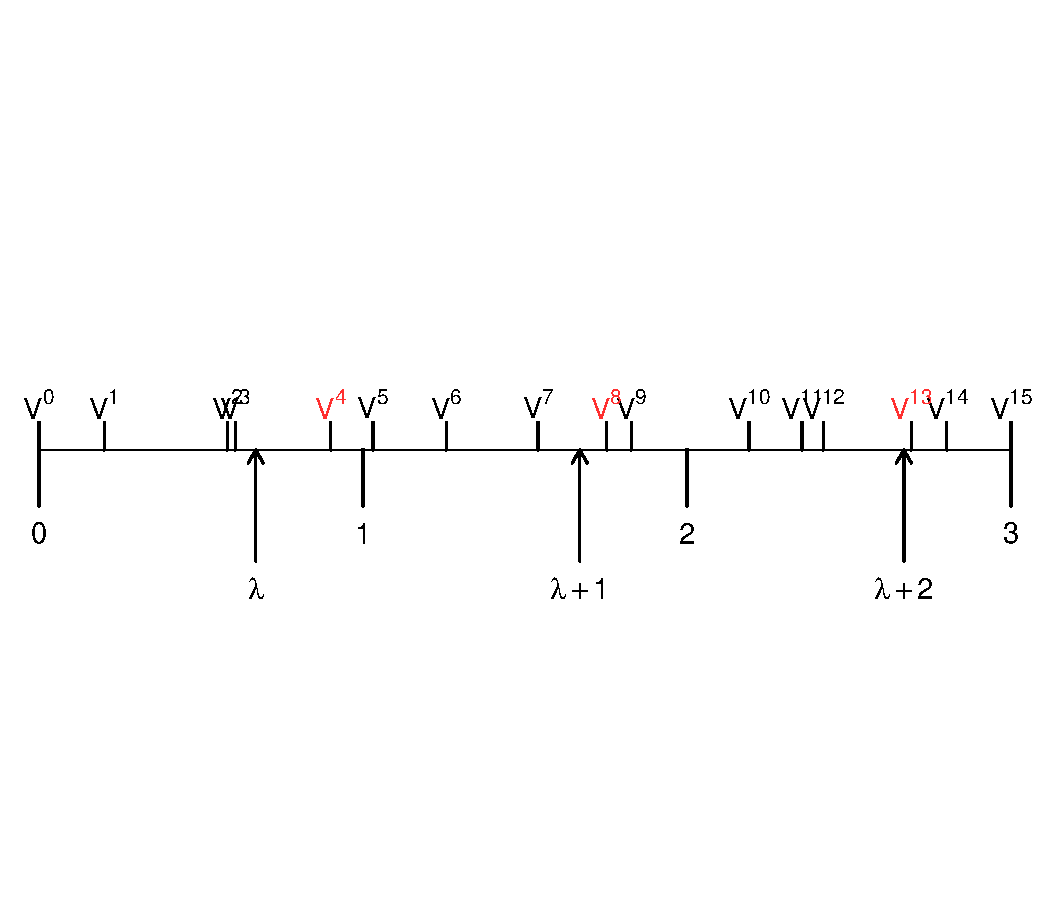
\includegraphics[width=.95\linewidth]{figure/UP_SYS-1} 

}



\end{knitrout}
~\\[-3cm]
Systematic selection remains popular because of its simplicity. Although unbiased variance estimation is in general not possible.
\end{frame}

\begin{frame}{Stratification}
A Population of 100 elements is stratified into $H=6$ strata.

%fig.keep='all',fig.show='asis'
\onslide*<1>{
\begin{knitrout}
\definecolor{shadecolor}{rgb}{0.969, 0.969, 0.969}\color{fgcolor}

{\centering 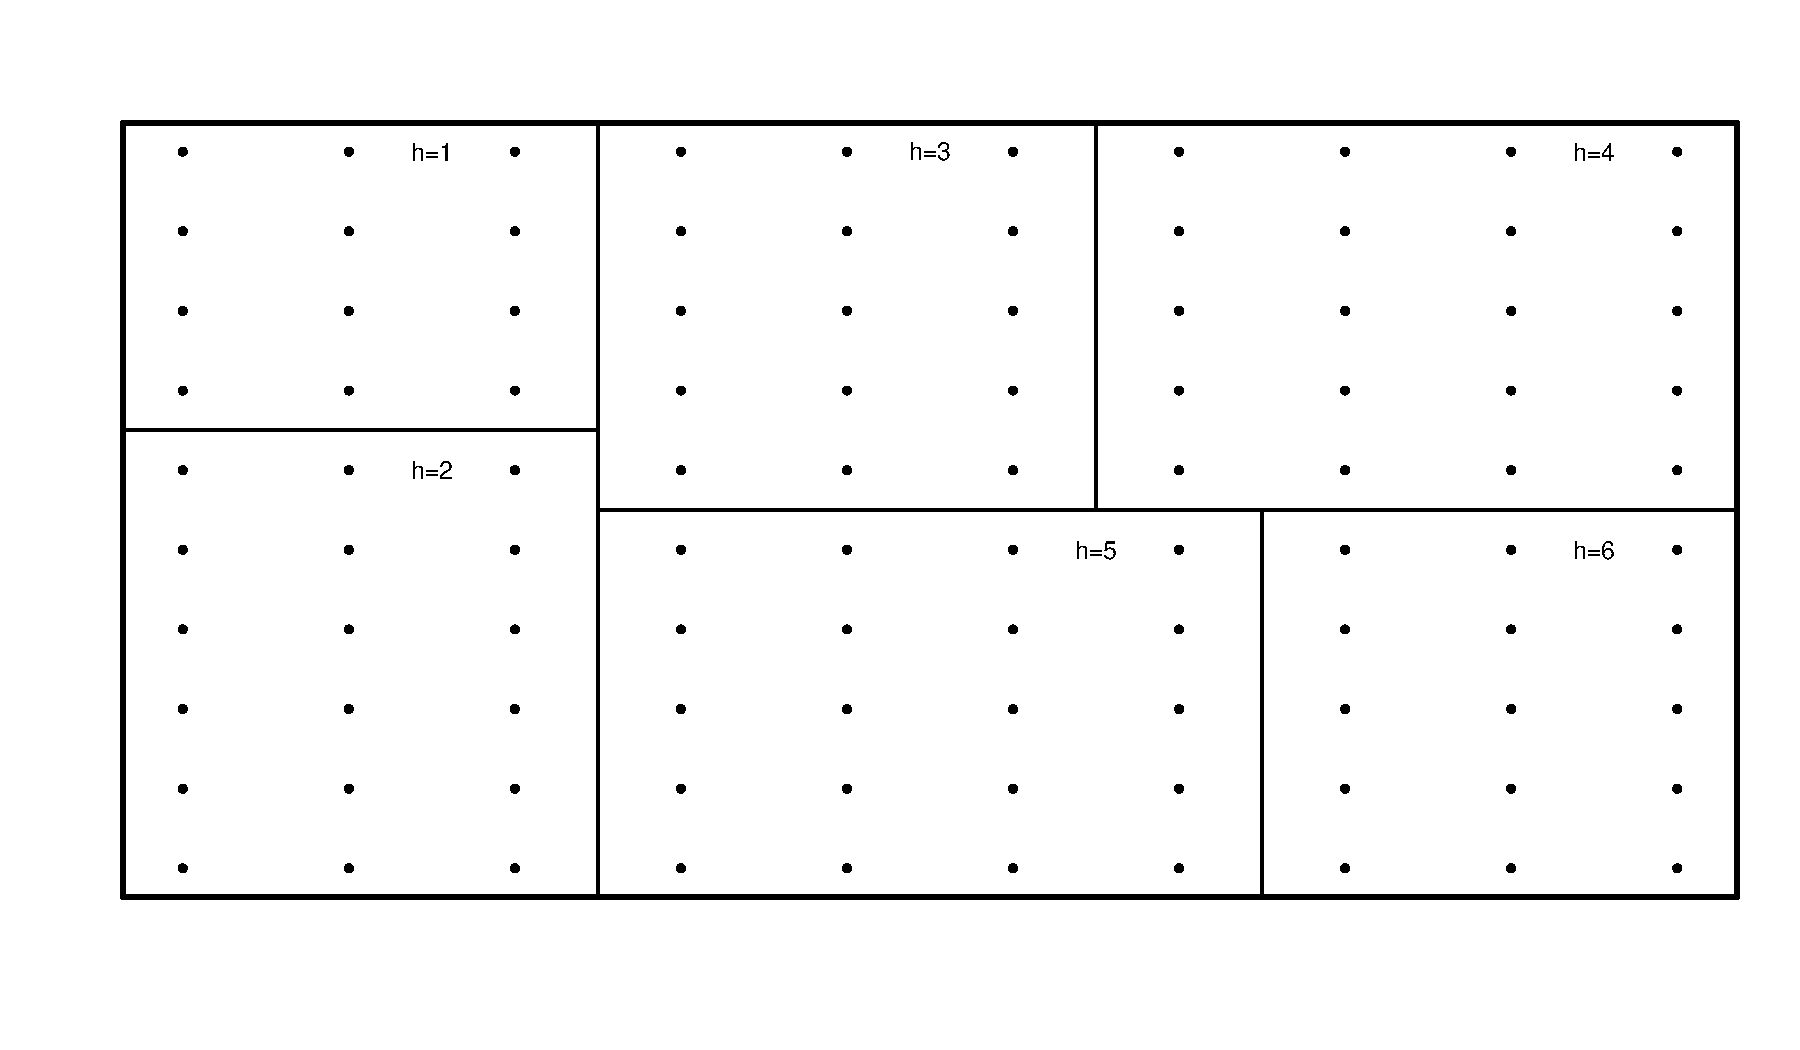
\includegraphics[width=.85\linewidth]{figure/StratPlot1-1} 

}



\end{knitrout}
}
\onslide<2>{
14 elements are selected population and their allocation is given by
\begin{tabular}{cccccc}
$n_1$ = 2  & $n_2$ = 3  & $n_3$ = 2  & $n_4$ = 3 & 
 $n_5$ = 3&  $n_6$ = 2\\
\end{tabular}

\begin{knitrout}
\definecolor{shadecolor}{rgb}{0.969, 0.969, 0.969}\color{fgcolor}

{\centering 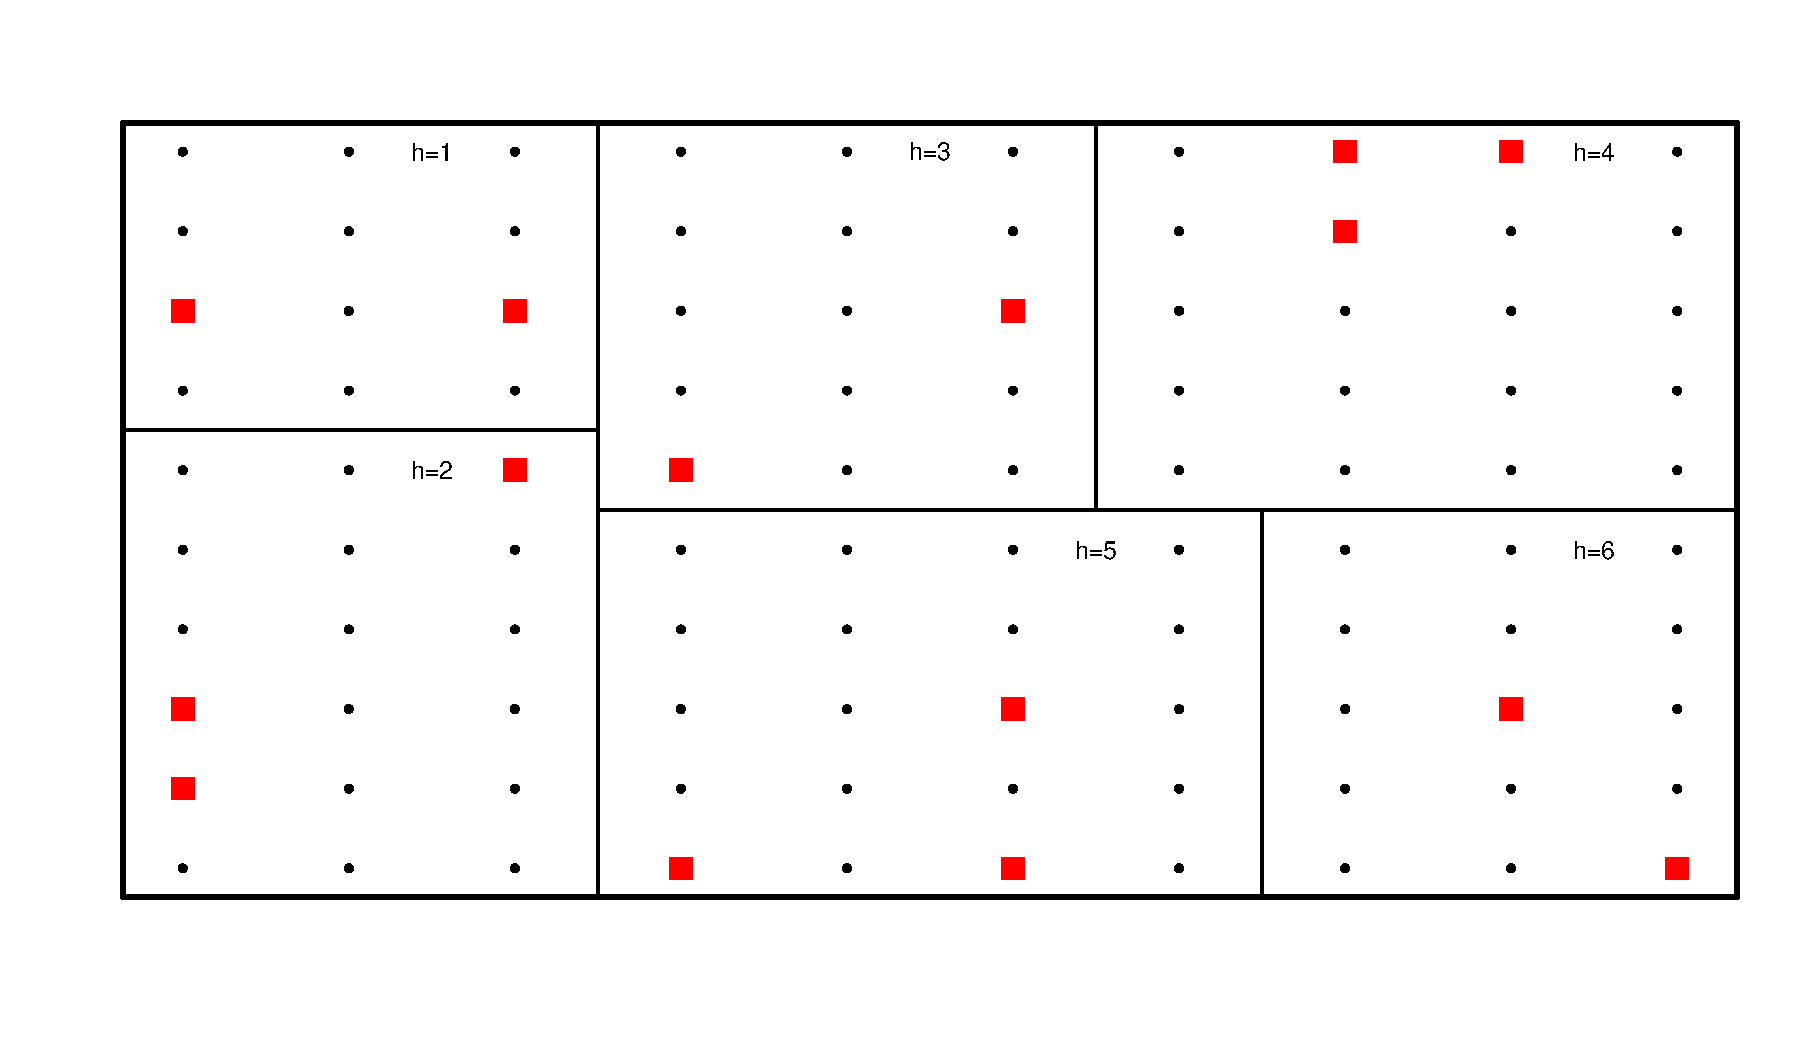
\includegraphics[width=.85\linewidth]{figure/StratPlot2-1} 

}



\end{knitrout}
}
\end{frame}


% \begin{frame}{Issues with Stratification}
% \begin{itemize}
% \item<1-> Why should stratification be used?
% \begin{itemize}
% \item<2-> To reduce the sampling variance of estimators.
% \item<2-> Sometimes it is necessary because of organizational reasons, (e.g. no joint sampling frame).
% \end{itemize}
% \item<3-> How should the population be stratified?
% \begin{itemize}
% \item<4-> A \emph{good} set of variables needs to be found for stratification.
% \item<4-> The number of strata has to be decided.
% \end{itemize}
% \item<5-> How should the overall sample size be allocated to the strata?
% \begin{itemize}
% \item<6-> Achieve proportionality between sample and population (i.e. the frame)
% \item<6-> Fulfill precision constraints for certain estimation domains
% \end{itemize}
% \end{itemize}
% 
% \end{frame}

\begin{frame}{Defining the Strata}
  \begin{table}\caption{Population ANOVA}
  \begin{tabular}{l | l | l }
  Source & df & Sum of Squares  \\
  \hline
   Between strata         & $H-1$ & $\text{SSB}  = \sum_{h=1}^H N_h ( \mu_{h} - \mu  )^2$  \\
   Within  strata         & $N-H$ & $\text{SSW}  = \sum_{h=1}^H (N_h-1) V_{h}^2$  \\
   Total,  about  $\mu_y$ & $N-1$ & $\text{SSTO} = (N-1) V^2$ \\
  \end{tabular}
  \end{table}
Stratification can reduce the sampling variance of estimators. The more homogeneous the strata are the higher is the gain in efficiency from using a stratified sample sample instead of SRS. That is if the SSW (variance within) is
considerably smaller that than the SSB (variance between). 
\end{frame}

\begin{frame}{Allocation Methods}
For all $h = 1{,}\,\ldots{,}\,H$
 \begin{equation*} \arraycolsep=1.4pt\def\arraystretch{2.2}
  n_h = \left\{ \begin{array}{l r}
        \dfrac{n}{H}  &\; \text{equal allocation} \\
        \dfrac{N_h}{N}  n    &\; \text{proportional allocation} \\
        \dfrac{N_h V_{h}}{\sum_{h=1}^H N_h V_{h} }  n  &\; \text{optimal allocation} 
  \end{array}\;\right.{,}
 \end{equation*}

Proportional allocation can also be done with respect to another variable, e.g. $\dfrac{\tau_h}{\tau}n$

% Variants of proportional allocation to totals
% proportional to y or auxiliar variable
% %the rounding probelem
\end{frame}

\begin{frame}[fragile]{Example Stratification}

\onslide*<1>{
We would like to estimate the difference in the mean Academic Performance Index (API) of all Californian schools between year 1999 and 2000 ($32.8$). To do that we select from all Californian schools two samples. One sample in 1999 and one in 2000. Both samples are selected by a  stratified (simple random) sample, where the Counties of California are used as the strata. The samples size for both samples is 205. From each County at least 2 schools are selected. The rest of the sampled size is allocated proportionally to the number of schools in the strata. The inclusion probability of a school in a particular stratum is the number of schools selected from that stratum divided by the total number of schools in that stratum. 
}
\onslide*<2>{
We use two estimator for variance estimation. One is design unbiased and the other is a naive estimator that uses no other design information than the design weights ($ \hat\sigma^2/n$).

% latex table generated in R 3.4.3 by xtable 1.8-2 package
% Mon Dec 11 23:09:05 2017
\begin{table}[ht]
\centering
\begin{tabular}{rrrrr}
  \hline
 & Est & Vest & CI.lb & CI.ub \\ 
  \hline
Design & 24.07 & 231.501 & -5.754 & 53.888 \\ 
  Naive & 24.07 & 190.810 & -3.007 & 51.141 \\ 
   \hline
\end{tabular}
\end{table}


The stratification seems to be not very effective. So we construct 10 strata that are more homogeneous with regard to $\text{API}_{99}$ and $\text{API}_{00}$ (using \emph{k-means}) and select two new samples.

% latex table generated in R 3.4.3 by xtable 1.8-2 package
% Mon Dec 11 23:09:05 2017
\begin{table}[ht]
\centering
\begin{tabular}{rrrrr}
  \hline
 & Est & Vest & CI.lb & CI.ub \\ 
  \hline
Design & 33.24 & 4.879 & 28.916 & 37.574 \\ 
  Naive & 33.24 & 165.890 & 8.001 & 58.489 \\ 
   \hline
\end{tabular}
\end{table}

} 

\onslide*<3>{
We repeat the sampling with the better stratification 1000 times and compute the coverage rates for our confidence intervals.

% latex table generated in R 3.4.3 by xtable 1.8-2 package
% Sun Dec 10 19:11:40 2017
\begin{table}[ht]
\centering
\begin{tabular}{rrr}
  \hline
 & Design & Naive \\ 
  \hline
Coverage Rate & 0.965 & 1.000 \\ 
   \hline
\end{tabular}
\end{table}

}

\end{frame}

\begin{frame}{Clustering}

A Population of 100 elements is clustered into $N_{\RN{1}}=6$ cluster
%fig.keep='all',fig.show='asis'
\onslide*<1>{
\begin{knitrout}
\definecolor{shadecolor}{rgb}{0.969, 0.969, 0.969}\color{fgcolor}

{\centering 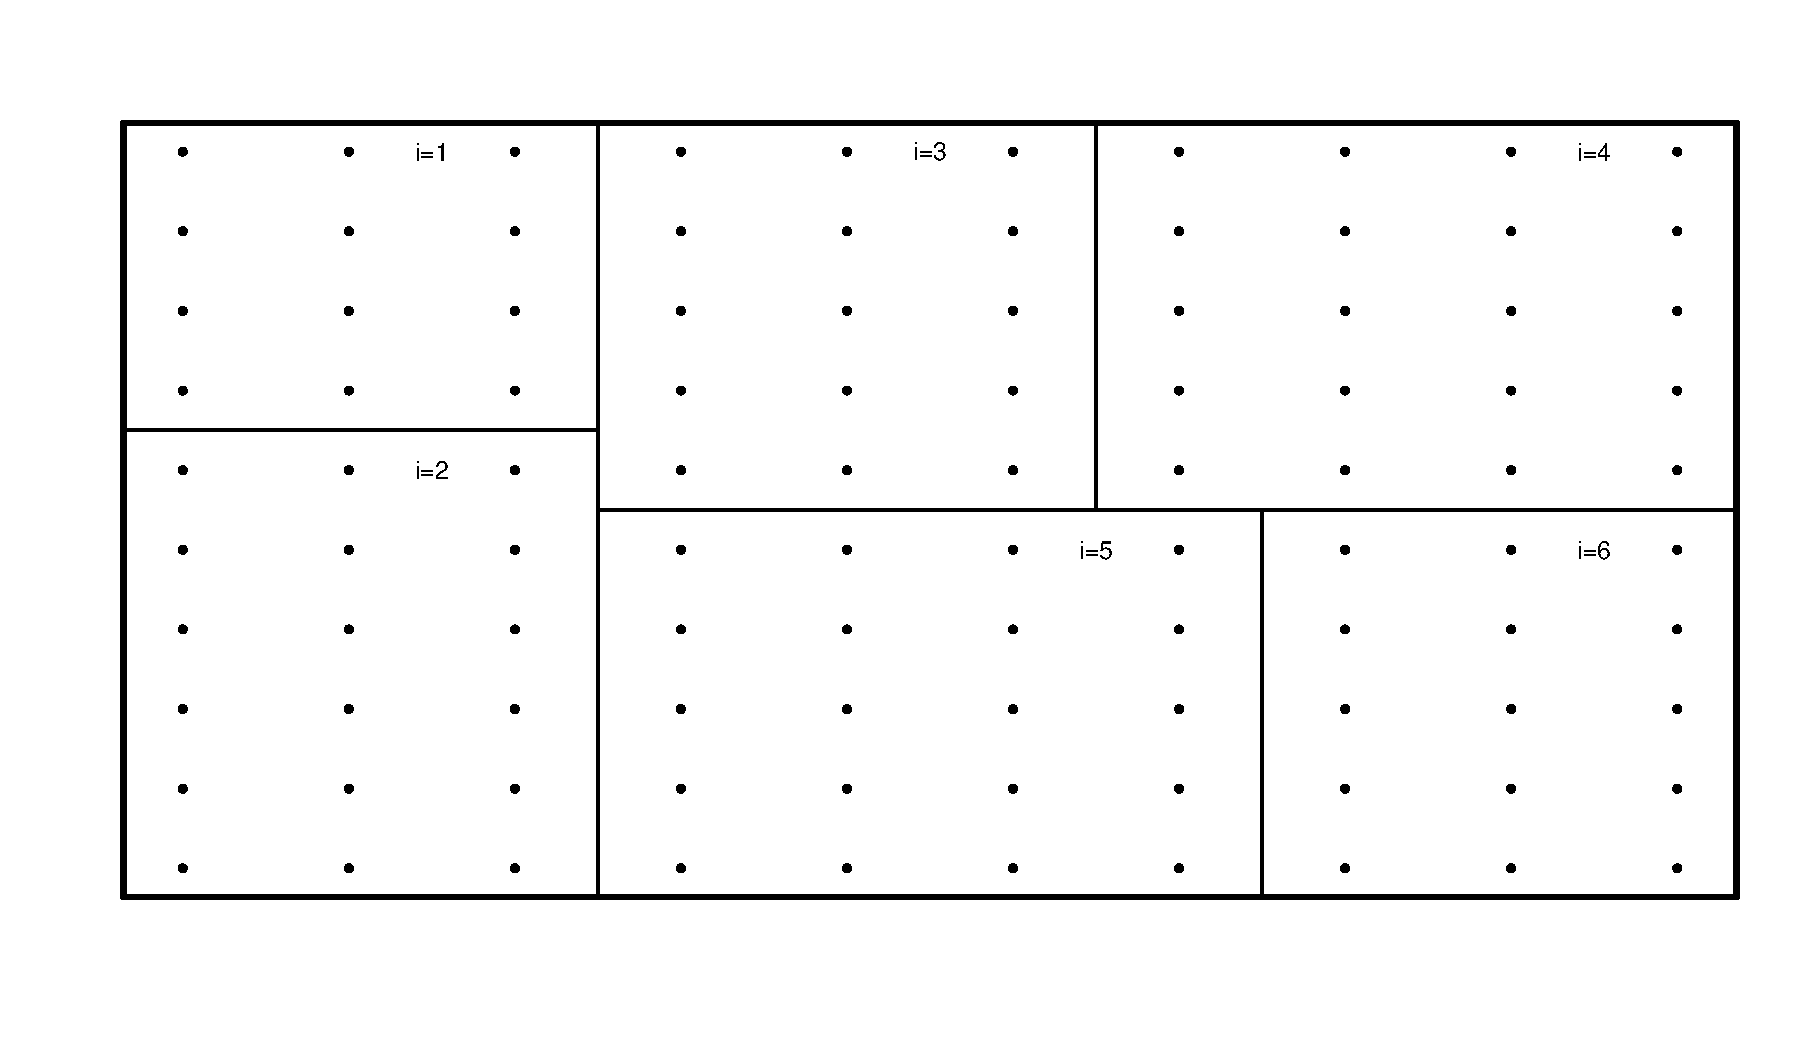
\includegraphics[width=.85\linewidth]{figure/CluPlot1-1} 

}



\end{knitrout}
}\onslide<2>{
and $n_{\RN{1}}=2$ clusters are selected from the population.
\begin{knitrout}
\definecolor{shadecolor}{rgb}{0.969, 0.969, 0.969}\color{fgcolor}

{\centering 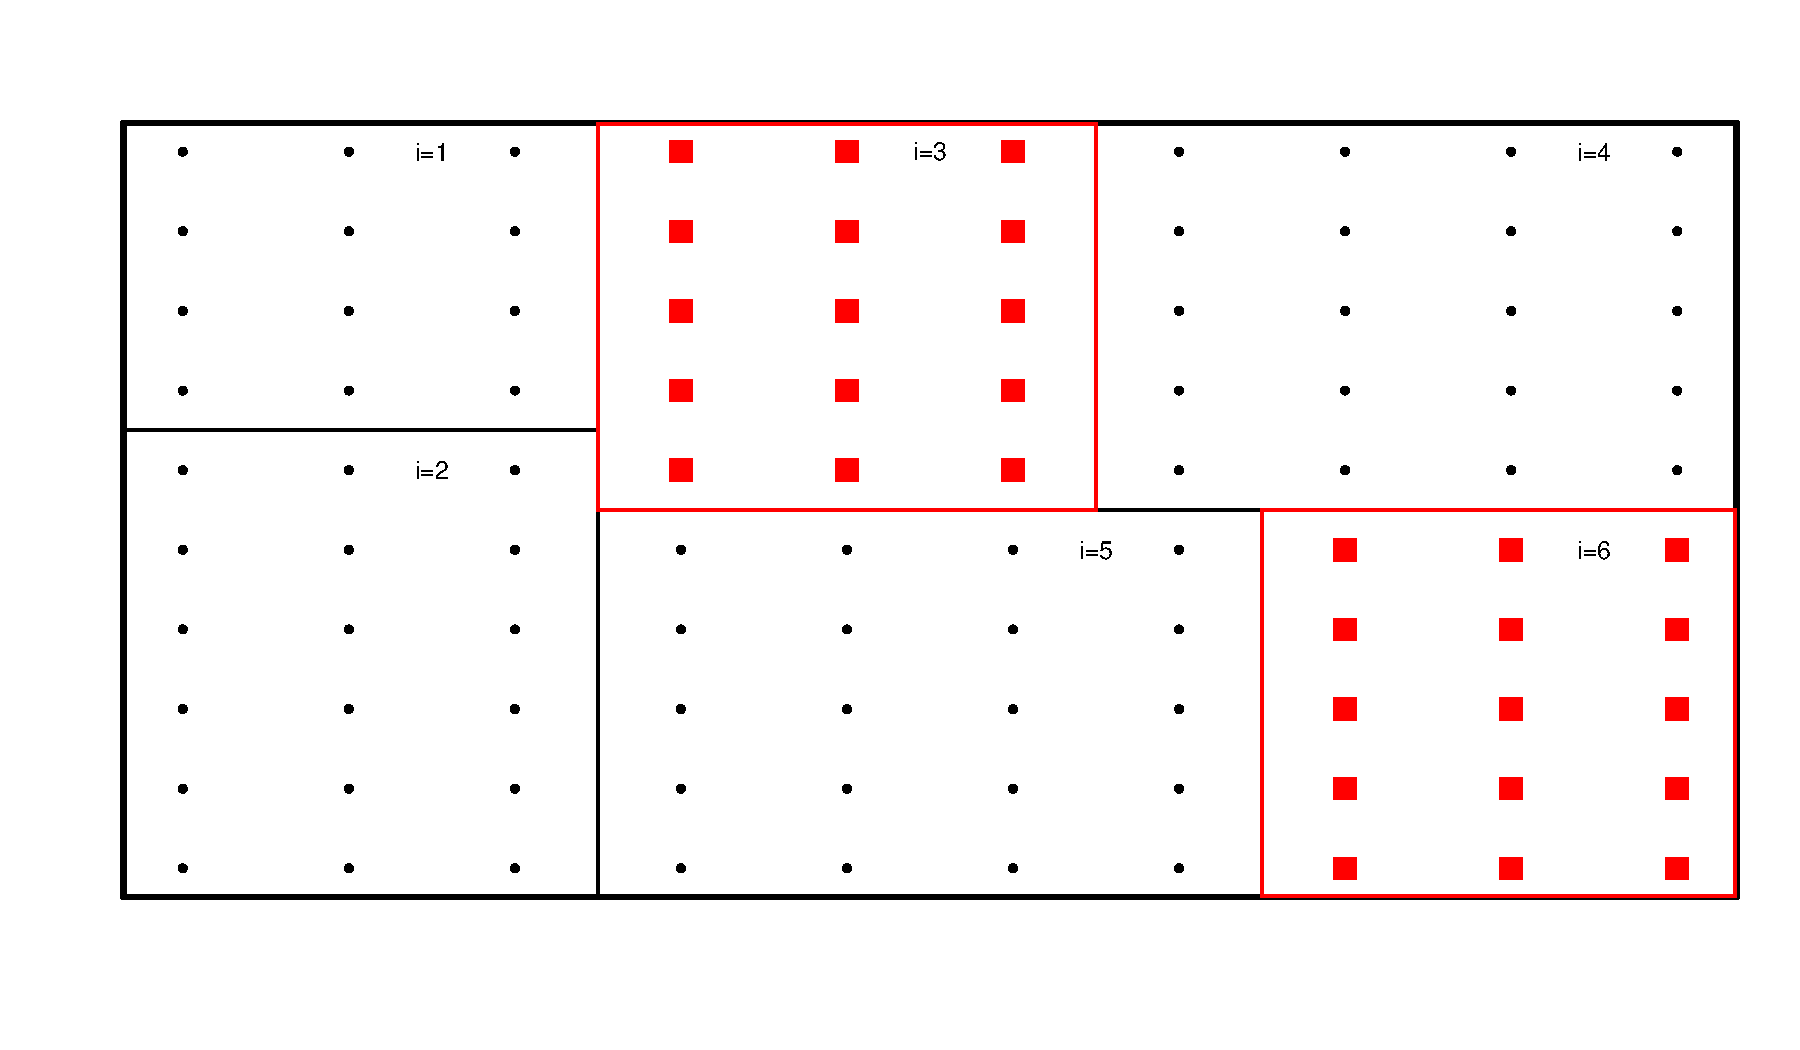
\includegraphics[width=.85\linewidth]{figure/CluPlot2-1} 

}



\end{knitrout}
}
\end{frame}


\begin{frame}{Cluster Sampling}
\onslide<1->{ Sampling elementary units is often not feasible (e.g. persons or businesses). Maybe there is no uniform sampling frame available to select them from, or it would be costly to do, because the selected elements would scatter to much over the a certain area and travel costs of interviewers would be to high. 
}
\onslide<2->{Thus, it is very common to select clusters, so called \emph{primary sampling units} (PSU's) that are populated by \emph{secondary sampling units} (SSU's).
}
\onslide<3->{Cluster sampling makes it still possible to obtain unbiased estimates but it can have a big influence on the variance. 
}
\onslide<4->{Compared to stratification cluster sampling tends to increase the sampling variance. What makes stratification efficient, a small within variance, has the opposite effect on cluster sampling.
}
\end{frame}



\begin{frame}[fragile]{Example Clustering}

\onslide*<1>{
Now we use for our Californian school survey cluster sampling. Both samples are selected by a (simple) cluster sample, where the clusters are the School Districts of California. 25 clusters are selected for both samples and the expected number of schools in each sample is $205$. Each cluster has the same inclusion probability, $0.0330251$ (25 divided by $757$, the number of clusters). 
}
\onslide*<2>{
We use two estimator for variance estimation. One is design unbiased and the other is a naive estimator that uses no other design information than the design weights ($\hat\sigma^2/n$).

% latex table generated in R 3.4.3 by xtable 1.8-2 package
% Mon Dec 11 23:09:06 2017
\begin{table}[ht]
\centering
\begin{tabular}{rrrrr}
  \hline
 & Est & Vest & CI.lb & CI.ub \\ 
  \hline
Design & 110.35 & 1755.376 & 28.229 & 192.463 \\ 
  Naive & 110.35 & 168.378 & 84.914 & 135.779 \\ 
   \hline
\end{tabular}
\end{table}


} 

\onslide*<3>{
We repeat the sampling 1000 times and compute the coverage rates for our confidence intervals.

% latex table generated in R 3.4.3 by xtable 1.8-2 package
% Sun Dec 10 19:29:37 2017
\begin{table}[ht]
\centering
\begin{tabular}{rrr}
  \hline
 & Design & Naive \\ 
  \hline
Coverage Rate & 0.863 & 0.415 \\ 
   \hline
\end{tabular}
\end{table}



Because of the under estimation by the naive variance estimator the naive approach results in a severe under coverage.
The design based approach does not under estimate the variance but their is a problem with the application of the CLT for building the confidence intervals.

}

\onslide*<4>{
We repeat the simulation, but only with 100 replications and this time we sample the clusters proportional to their number of schools. Thus the inclusion probability of each cluster is $\dfrac{N_i}{N}*25$, where $N_i$ is the number of schools in the $i$-th cluster and N the total number of schools ($6194$).

% latex table generated in R 3.4.3 by xtable 1.8-2 package
% Mon Dec 11 22:20:12 2017
\begin{table}[ht]
\centering
\begin{tabular}{rrr}
  \hline
 & Design & Naive \\ 
  \hline
Coverage Rate & 0.980 & 0.330 \\ 
   \hline
\end{tabular}
\end{table}

}

\end{frame}



%\section{Complex Sampling Designs - Two Stage Sampling}

\begin{frame}{Two Stage Sampling}
% A Population of 100 elements is clustered into $N_{\RN{1}}=6$ clusters
% and $n_{\RN{1}}=n_I$ clusters (PSU) are selected at the first sampling stage
\onslide*<1>{
\begin{knitrout}
\definecolor{shadecolor}{rgb}{0.969, 0.969, 0.969}\color{fgcolor}

{\centering 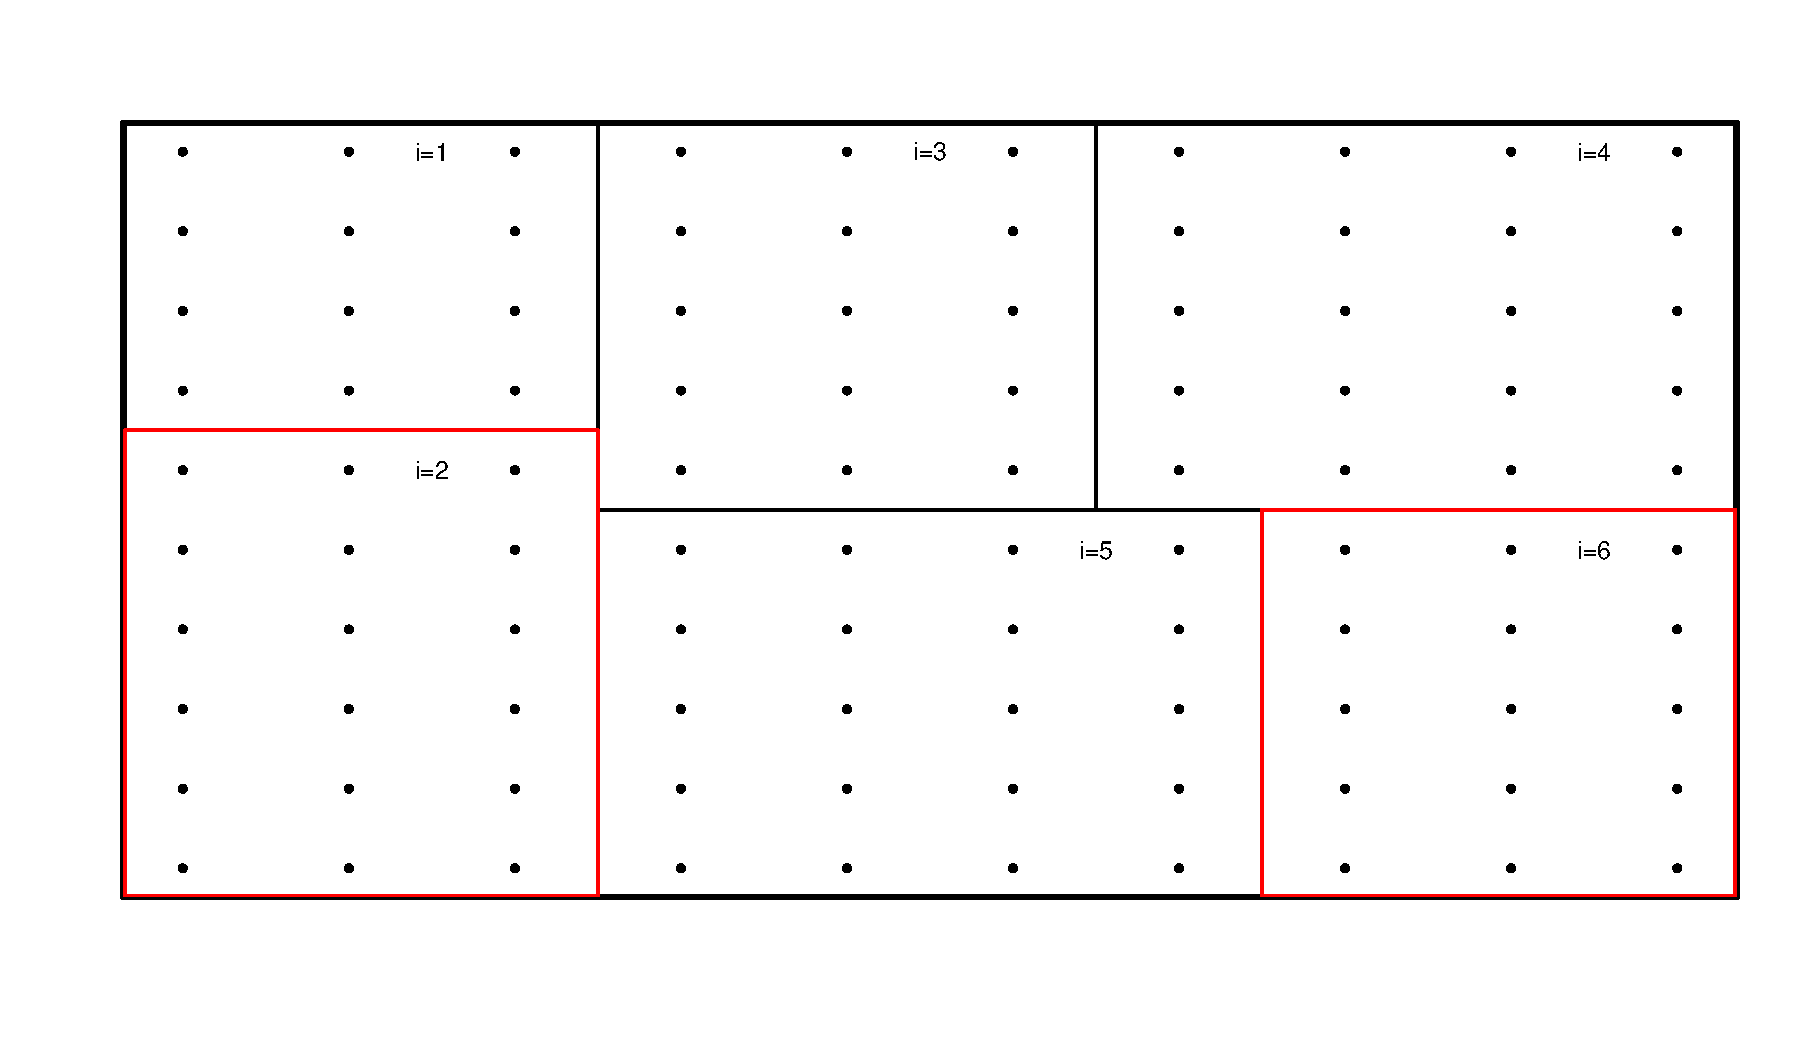
\includegraphics[width=.85\linewidth]{figure/CluPlot1_2-1} 

}



\end{knitrout}

}\onslide<2>{
and $n_{i}=4$ elements are selected from each sampled cluster.
\begin{knitrout}
\definecolor{shadecolor}{rgb}{0.969, 0.969, 0.969}\color{fgcolor}

{\centering 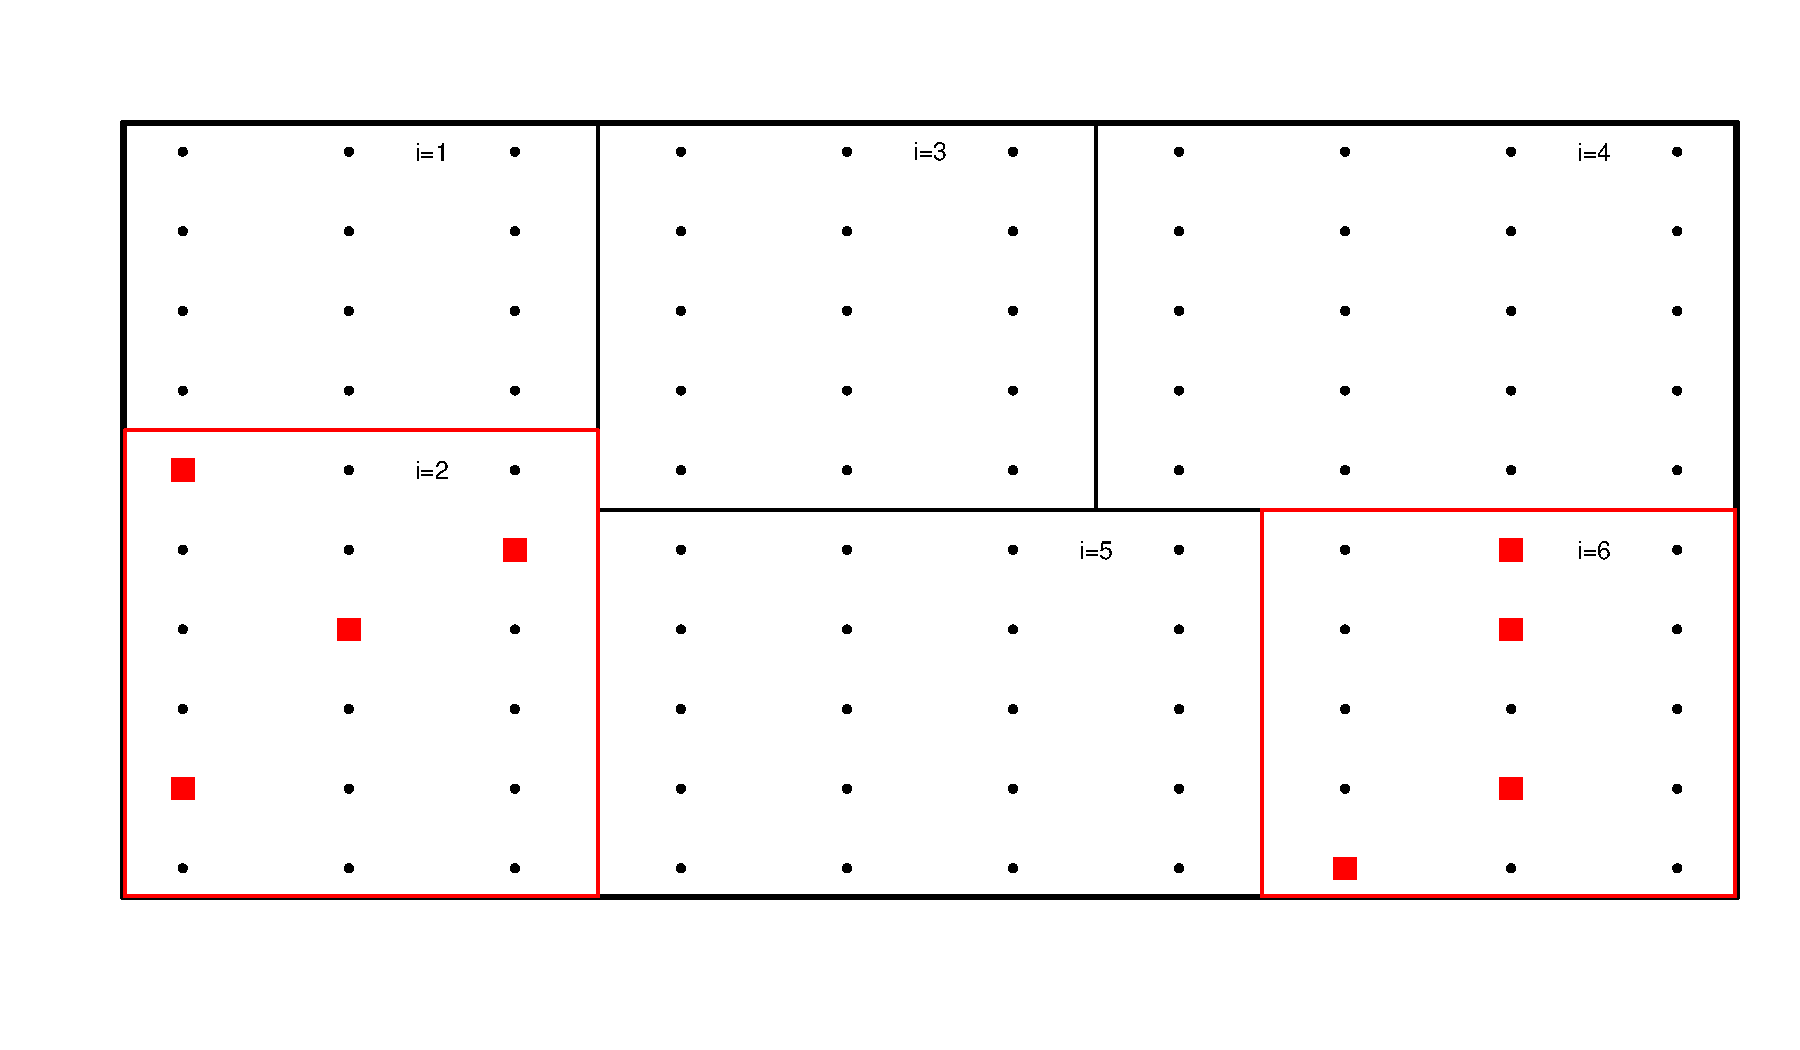
\includegraphics[width=.85\linewidth]{figure/CluPlot2_2-1} 

}



\end{knitrout}
}





\end{frame}


\begin{frame}{Two Stage Sampling}
 \begin{description}
 \item[First  stage] A sample $\mathfrc{s}_{\RN{1}}$ of PSU's is drawn from $\mathcal{U}_{\RN{1}}$ according to some sampling design $p_{\RN{1}}(.)$
 \item[Second stage] For every $i \in \mathfrc{s}_{\RN{1}}$ a sample $\mathfrc{s}_i$ of SSU's is selected from $\mathcal{U}_i$ according to some design $p_i(.|\mathfrc{s}_{\RN{1}})$
 \end{description}
 The resulting sample of SSU's is denote $\mathfrc{s}= \bigcup_{i \in \mathfrc{s}_{\RN{1}}} \mathfrc{s}_i $.
 In general, samples $\mathfrc{s}_i$ are selected independently of each other, thus, the inclusion probability of a element $k \in \mathcal{U}_i$ is
$$\pi_k=\pi_{\RN{1}i}\pi_{k|i}\;,$$
where $\pi_{\RN{1}i}$ is the probability of selecting the $i$-th PSU and $\pi_{k|i}$  the probability of selecting
the $k$-th SSU within the $i$-th PSU.
\end{frame}



\begin{frame}[fragile]{Example Two Stage Sampling}

\onslide*<1>{
For our Californian schools would like to estimate the following model $\text{API}_{00} = \text{ell}+\text{meals}+\text{mobility}+\text{stype}$,
where
\begin{itemize}
\item[ell] = English Language Learners (percent)
\item[meals] =  Percentage of students eligible for subsidized meals,
\item[mobility] = percentage of students for whom this is the first year at the school,
\item[stype] = Elementary/Middle/High School
\end{itemize}
Now we use a two stage sample. As PSUs the counties of California are used, the SSU are the schools. 25 PSUs are selected with probablity proportional to their number of schools. Within each selected PSU 2 schools are sampled by a SRS.
 }
\onslide<2>{

% latex table generated in R 3.4.3 by xtable 1.8-2 package
% Mon Dec 11 23:09:06 2017
\begin{table}[ht]
\centering
\caption{Naive} 
\scalebox{0.6}{
\begin{tabular}{rrrrr}
  \hline
 & Estimate & Std. Error & t value & Pr($>$$|$t$|$) \\ 
  \hline
(Intercept) & 853.819 & 24.221 & 35.251 & 0.000 \\ 
  ell & -1.475 & 0.616 & -2.394 & 0.021 \\ 
  meals & -3.217 & 0.460 & -6.999 & 0.000 \\ 
  mobility & 1.173 & 1.368 & 0.858 & 0.396 \\ 
  stypeH & -110.767 & 23.125 & -4.790 & 0.000 \\ 
  stypeM & 7.754 & 45.369 & 0.171 & 0.865 \\ 
   \hline
\end{tabular}
}
\end{table}
% latex table generated in R 3.4.3 by xtable 1.8-2 package
% Mon Dec 11 23:09:06 2017
\begin{table}[ht]
\centering
\caption{Design} 
\scalebox{0.6}{
\begin{tabular}{rrrrr}
  \hline
 & Estimate & Std. Error & t value & Pr($>$$|$t$|$) \\ 
  \hline
(Intercept) & 853.819 & 25.084 & 34.039 & 0.000 \\ 
  ell & -1.475 & 0.626 & -2.356 & 0.036 \\ 
  meals & -3.217 & 0.409 & -7.866 & 0.000 \\ 
  mobility & 1.173 & 1.257 & 0.933 & 0.369 \\ 
  stypeH & -110.767 & 49.419 & -2.241 & 0.045 \\ 
  stypeM & 7.754 & 46.304 & 0.167 & 0.870 \\ 
   \hline
\end{tabular}
}
\end{table}

}
\end{frame}


\section{Sample Size Planning}

\begin{frame}{Selecting a Sample Size}
\onslide*<1>{
The sample size can be set to achieve a desired level of precision in terms of the variance 
$\V{\hat{\theta}}$ or the variation coefficient $\text{CV}(\hat{\theta})  = \frac{\sqrt{\text{V}(\hat{\theta})}}{\hat{\theta}}$. \newline
Set $\text{CV}(\overline{y}) = \text{CV}_0$ as a precision requirement (representative!).
\begin{align}
n & = \dfrac{ V^2  \mu^{-2}}{\text{CV}_0^2 +  V^2  N^{-1} \mu^{-2}} \eqname{SRS} 
 \end{align}
}
\onslide*<2>{
There are many ways to optimize the sampling design with
respect to one particular goal, i.e. the estimation of a specific
statistic. However, it becomes difficult to optimize a design and at
the same time retain a balance for a maximum of possible
applications, which is a problem when planning a multipurpose
survey that has a multitude of variables and covers different
topics. Thus simple design, such as SRS or stratified SRS, are
justifiable, as these designs are robust towards any possible
analysis of the sample data.
}
\end{frame}

\begin{frame}{Sample Size for Proportions}
\onslide*<1,3>{If the variable of interest is binary we have $\V{\overline{y}}_{\text{SRS}} = \dfrac{\mu(1-\mu) }{n} \dfrac{N-n}{N-1}$ and $\text{CV}^2(\overline{y})_\text{SRS}=\left( \dfrac{1}{n} - \dfrac{1}{N}\right) \dfrac{N}{N-1} \dfrac{(1-\mu)}{\mu}$. However $ \lim_{\mu \to 0} \text{CV}^2(\overline{y})_\text{SRS} = \infty\;$, thus for rare observation to meet a CV target the sample size can become very large.
}
\onslide*<2>{
\begin{knitrout}
\definecolor{shadecolor}{rgb}{0.969, 0.969, 0.969}\color{fgcolor}\begin{figure}

{\centering 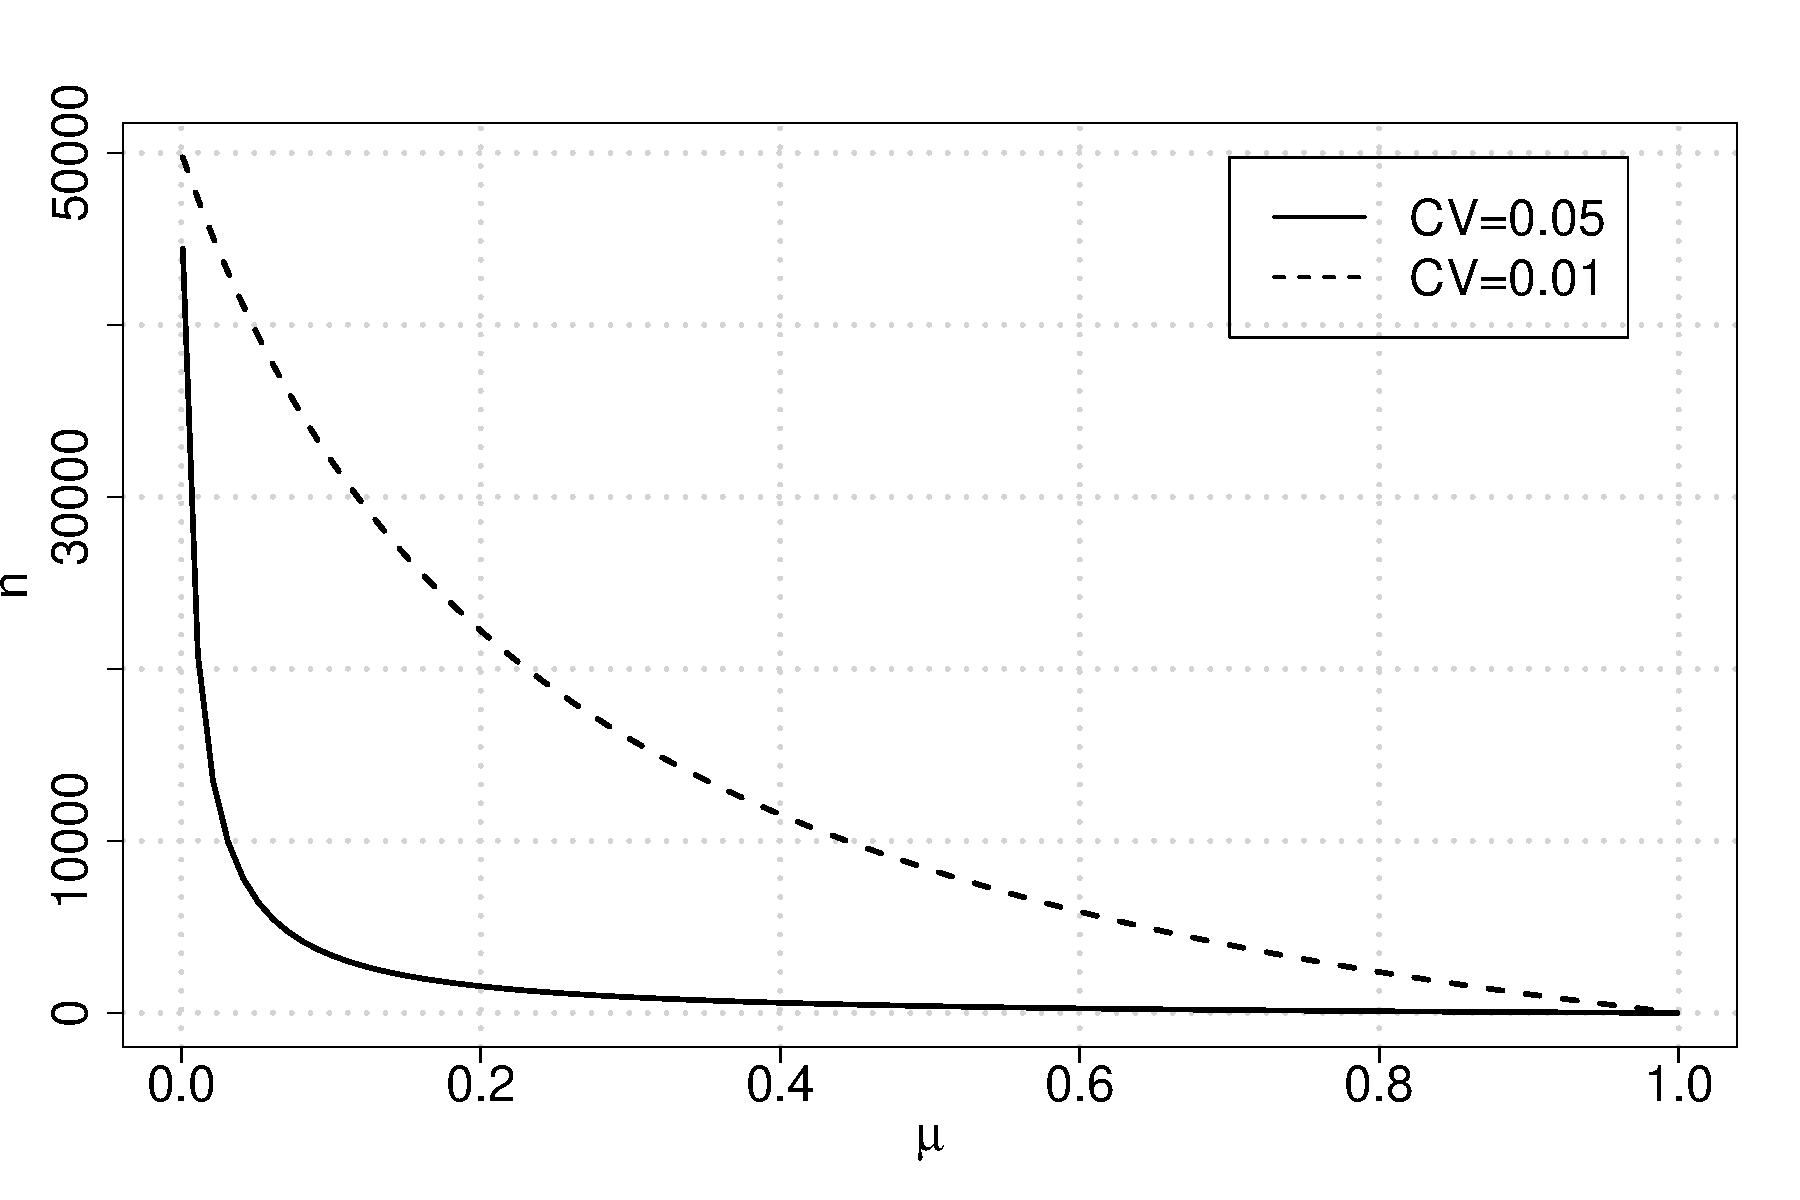
\includegraphics[width=.85\linewidth]{figure/SamSizeSRSprobs-1} 

}

\caption[Sample Sizes to Achieve CV's of 0.05 and 0.01 for N=50000]{Sample Sizes to Achieve CV's of 0.05 and 0.01 for N=50000}\label{fig:SamSizeSRSprobs}
\end{figure}


\end{knitrout}
}
\onslide*<3>{The target for $\V{\overline{y}}_{\text{SRS}}$ can be set to achieve a CI's with a maximal length of $2\epsilon$.
% \begin{align*}
% \epsilon \geq & z_{1-\alpha/2} \sqrt{ \dfrac{\mu(1-\mu) }{n} \dfrac{N-n}{N-1} } &
% n \geq & \dfrac{ z_{1-\alpha/2}^2 \frac{N}{N-1} \mu(1-\mu) }{\epsilon^2  + \frac{1}{N}  z_{1-\alpha/2}^2 \frac{N}{N-1} \mu(1-\mu) }
% \end{align*}
}
\onslide*<4>{
\begin{knitrout}
\definecolor{shadecolor}{rgb}{0.969, 0.969, 0.969}\color{fgcolor}\begin{figure}

{\centering 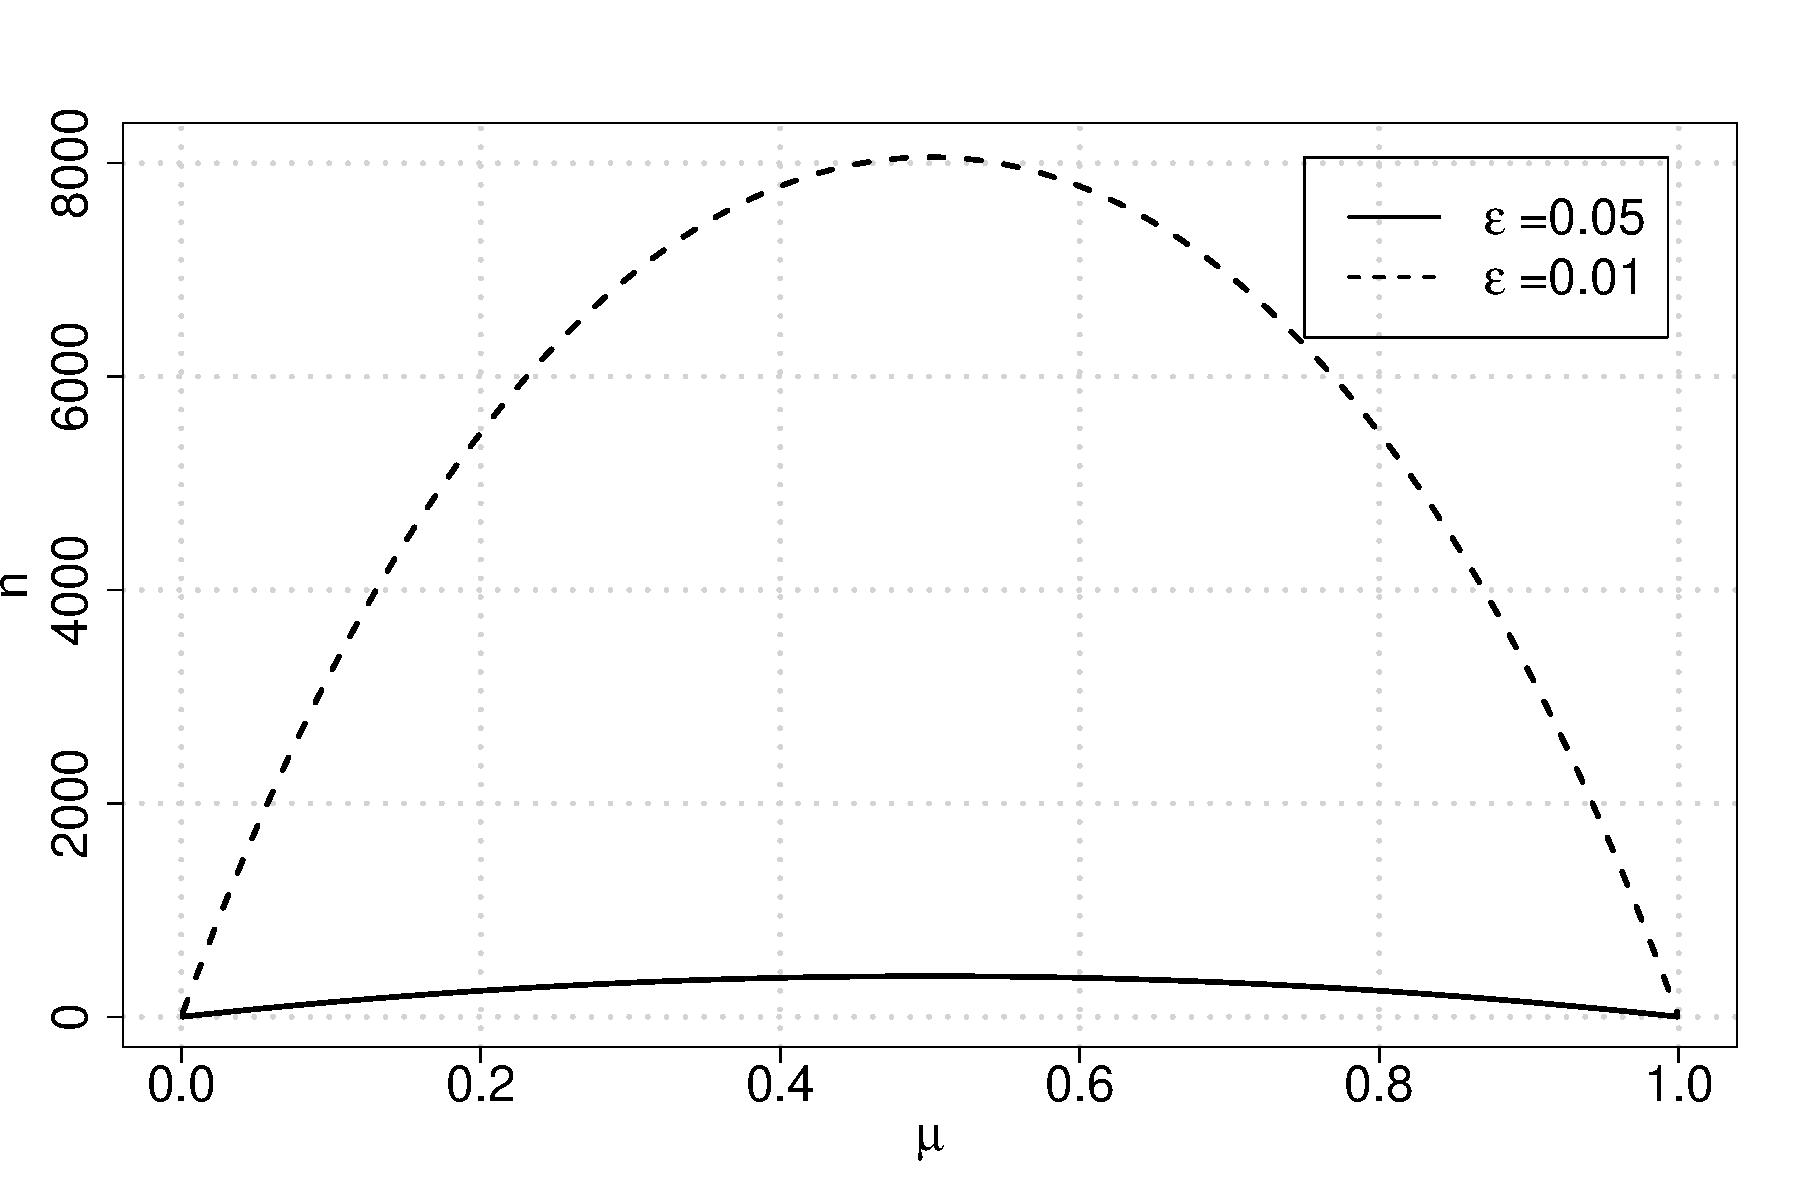
\includegraphics[width=.85\linewidth]{figure/SamSizeSRSprobs2-1} 

}

\caption[Sample Sizes to Achieve Absolute Errors of 0.05 and 0.01 for N=50000]{Sample Sizes to Achieve Absolute Errors of 0.05 and 0.01 for N=50000}\label{fig:SamSizeSRSprobs2}
\end{figure}


\end{knitrout}
}
\end{frame}

\begin{frame}[allowframebreaks]\frametitle{Literature}    
%\scriptsize
  \begin{thebibliography}{10}    
   \setbeamertemplate{bibliography item}[book]
   \bibitem{Lohr1999}
    S.~Lohr.
    \newblock  Sampling: Design and Analysis.
    \newblock {\em Duxbury Press}, 1999.
   \setbeamertemplate{bibliography item}[book]
  \bibitem{Lumley2010}
    T.~Lumley.
    \newblock Complex Surveys: A Guide to Analysis Using R.
    \newblock {\em Wiley}, 2010.
   \setbeamertemplate{bibliography item}[book]
  \bibitem{Saerndal1992}
    C.-E.~S\"{a}rndal, B.~Swensson, \& J.~Wretman.
    \newblock Model Assisted Survey Sampling
    \newblock {\em Springer}, 1992.
    \setbeamertemplate{bibliography item}[book]
  \bibitem{Tille2006}
   Y.~Till\'{e}.
  \newblock  Sampling Algorithms
    \newblock {\em Springer Series in Statistics: Springer}, 2006.
  \end{thebibliography}
\end{frame} 


\end{document} 
